

We compare our method \gls{MLD} to \gls{MVAE} \cite{mvaeWu2018}, \gls{MMVAE} \cite{mmvaeShi2019}, \gls{MOPOE} \cite{sutter2021generalized}, \gls{NEXUS} \cite{Vasco2022} and \gls{MVTCAE} \cite{tcmvaehwang21}, \gls{MMVAEplus} \cite{palumbo2023mmvae} re-implementing competitors in the same code base as our method, and selecting their best hyper-parameters (as indicated by the authors). For fair comparison, we use the same encoder/decoder architecture for all the models. For \gls{MLD}, the score network is implemented using a simple stacked \gls{MLP} with skip connections (see \ref{apdx:mld_details} for more details).



\noindent \textbf{Evaluation metrics.} \textit{Coherence} is measured as in \cite{mmvaeShi2019, sutter2021generalized, palumbo2023mmvae}, using pre-trained classifiers on the generated data and checking the consistency of their outputs. \textit{Generative quality} is computed using \gls{FID} \cite{fid} and \gls{FAD} \cite{fad} scores for images and audio respectively. Full details on the metrics are included in \ref{apdx:dataset_eval}. All results are averaged over 5 seeds (We report standard deviation in \ref{apdx:additionnal_res}).





\noindent \textbf{Results.} Overall, \gls{MLD} largely outperforms alternatives from the literature, \textbf{both} in terms of coherence and generative quality. \gls{VAE}-based models suffer from a coherence--quality trad-off and modality collapse for highly heterogeneous data-sets. We proceed to show this on several standard benchmarks from the multi-modal \gls{VAE}-based literature (see \ref{apdx:dataset_eval} for details on the data-sets).



The first data-set we consider is \textbf{\mnist-\svhn} (\citep{mmvaeShi2019}), where the two modalities differ in complexity.  
High variability, noise and ambiguity makes attaining good coherence for the \svhn modality a challenging task. Overall, \gls{MLD} outperforms all \gls{VAE}-based alternatives in terms of coherency, especially in terms of joint generation and conditional generation of \mnist given \svhn, see \Cref{coh_quality:ms}. Mixture models (\gls{MMVAE}, \gls{MOPOE}) suffer from modality collapse (poor \svhn generation), whereas product of experts (\gls{MVAE}, \gls{MVTCAE}) generate better quality samples at the expense of \svhn to \mnist conditional coherence. Joint generation is poor for all \gls{VAE} models. Interestingly, these models also fail at \svhn self-reconstruction which we discuss in \ref{apdx:additionnal_res}. \gls{MLD} achieves the best performance also in terms of generation quality, as confirmed also by qualitative results (\Cref{fig:cond_joint_ms}) showing for example how \gls{MLD} conditionally generates multiple \svhn digits within one sample, given the input \mnist image, whereas other methods fail to do so. 








\begin{table}[h]
\caption{Generation coherence and quality for \textbf{\mnist-\svhn} ( M :\mnist, S: \svhn ). The generation quality is measured in terms of \gls{FMD}  for \mnist and \gls{FID} for \svhn.}
\centering
\tiny
\begin{tabular}{c|c|cc|cc|cc}
\toprule
\multirow{2}{*}{ Models }  & \multicolumn{3}{c}{Coherence (\%$\uparrow$) } &   \multicolumn{4}{c}{Quality ($\downarrow$)} \\
    \cmidrule{2-8}
    & Joint &  M $\rightarrow$ S & S $\rightarrow$ M &
     Joint(M)  &  Joint(S) &M $\rightarrow$ S &  S $\rightarrow$ M  \\
    \midrule
     \gls{MVAE} &  
     $38.19$ &
     $48.21$  &
     $ 28.57$ & 
     $13.34$ &
     $68.9$   & 
     $ \underline{68.0}  $ &
     $ 13.66 $ 
    
     \\
    \gls{MMVAE} &  $37.82$ & $11.72$ & $ 67.55$ & $25.89$ &
    $ 146.82  $& $393.33$  &
    $ 53.37 $ 
 
    \\
    \gls{MOPOE} & $ 39.93$ & $12.27$ & $68.82$ &$20.11$ &
    $ 129.2  $&$373.73$&
    $ 43.34 $
        \\

    \gls{NEXUS} &  $ 40.0$ & $16.68$ & $\underline{70.67}$ &  $13.84$ &
        $ 98.13  $ &$281.28$&
 $ 53.41 $
   \\


    \gls{MVTCAE} & $\underline{48.78} $& $\underline{81.97}$ & $49.78 $&$\underline{12.98}$ &
    $ \textbf{52.92} $&$69.48$ &
    $ \underline{13.55} $ 
\\ 
\gls{MMVAEplus} &17.64 &13.23 & 29.69 &26.60 & 121.77 & 240.90&35.11
\\
  \gls{MMVAEplus}(K=10) & 41.59 & 55.3
& 56.41 & 19.05 & 67.13 & 75.9 & 18.16






      \\
     
    \midrule
    \textbf{\gls{MLD} (ours)}  & $\textbf{85.22}$ & 
    $\textbf{83.79} $&
    $ \textbf{79.13}$ &
    $\textbf{3.93}$ &
    $\underline{56.36}$   &
    $\textbf{57.2}$  &
    $\textbf{3.67} $ 
    \\
    \bottomrule
   
\end{tabular}
\label{coh_quality:ms}
\end{table}




\begin{figure}[h]
     \centering

\begin{subfigure}{0.15\textwidth}
         \centering
         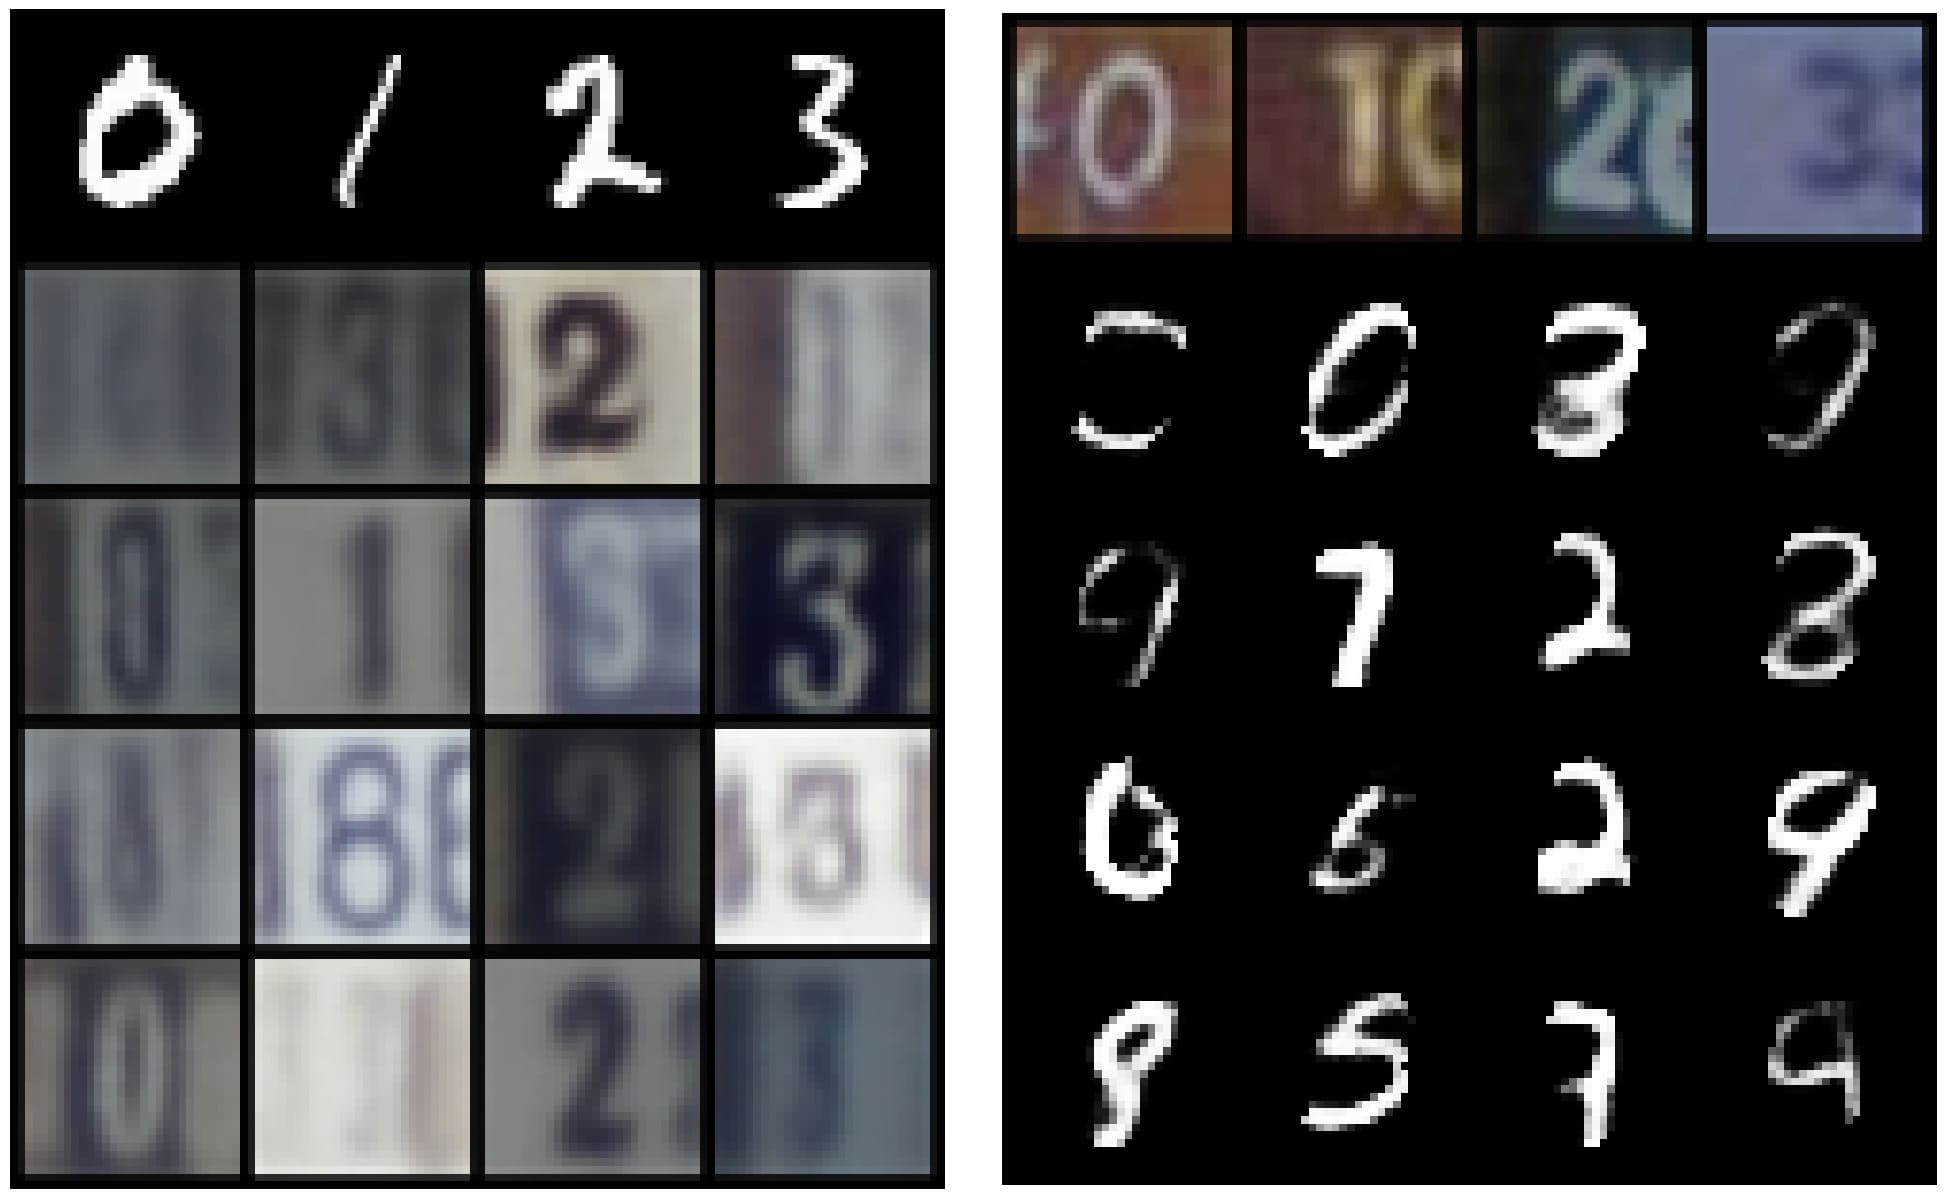
\includegraphics[width=\linewidth]{figures/datasets/ms/smallmvae_cond_mnist_svhn.jpg}
    
\caption*{\gls{MVAE}}      
\end{subfigure}
\begin{subfigure}{0.15\textwidth}
         \centering
         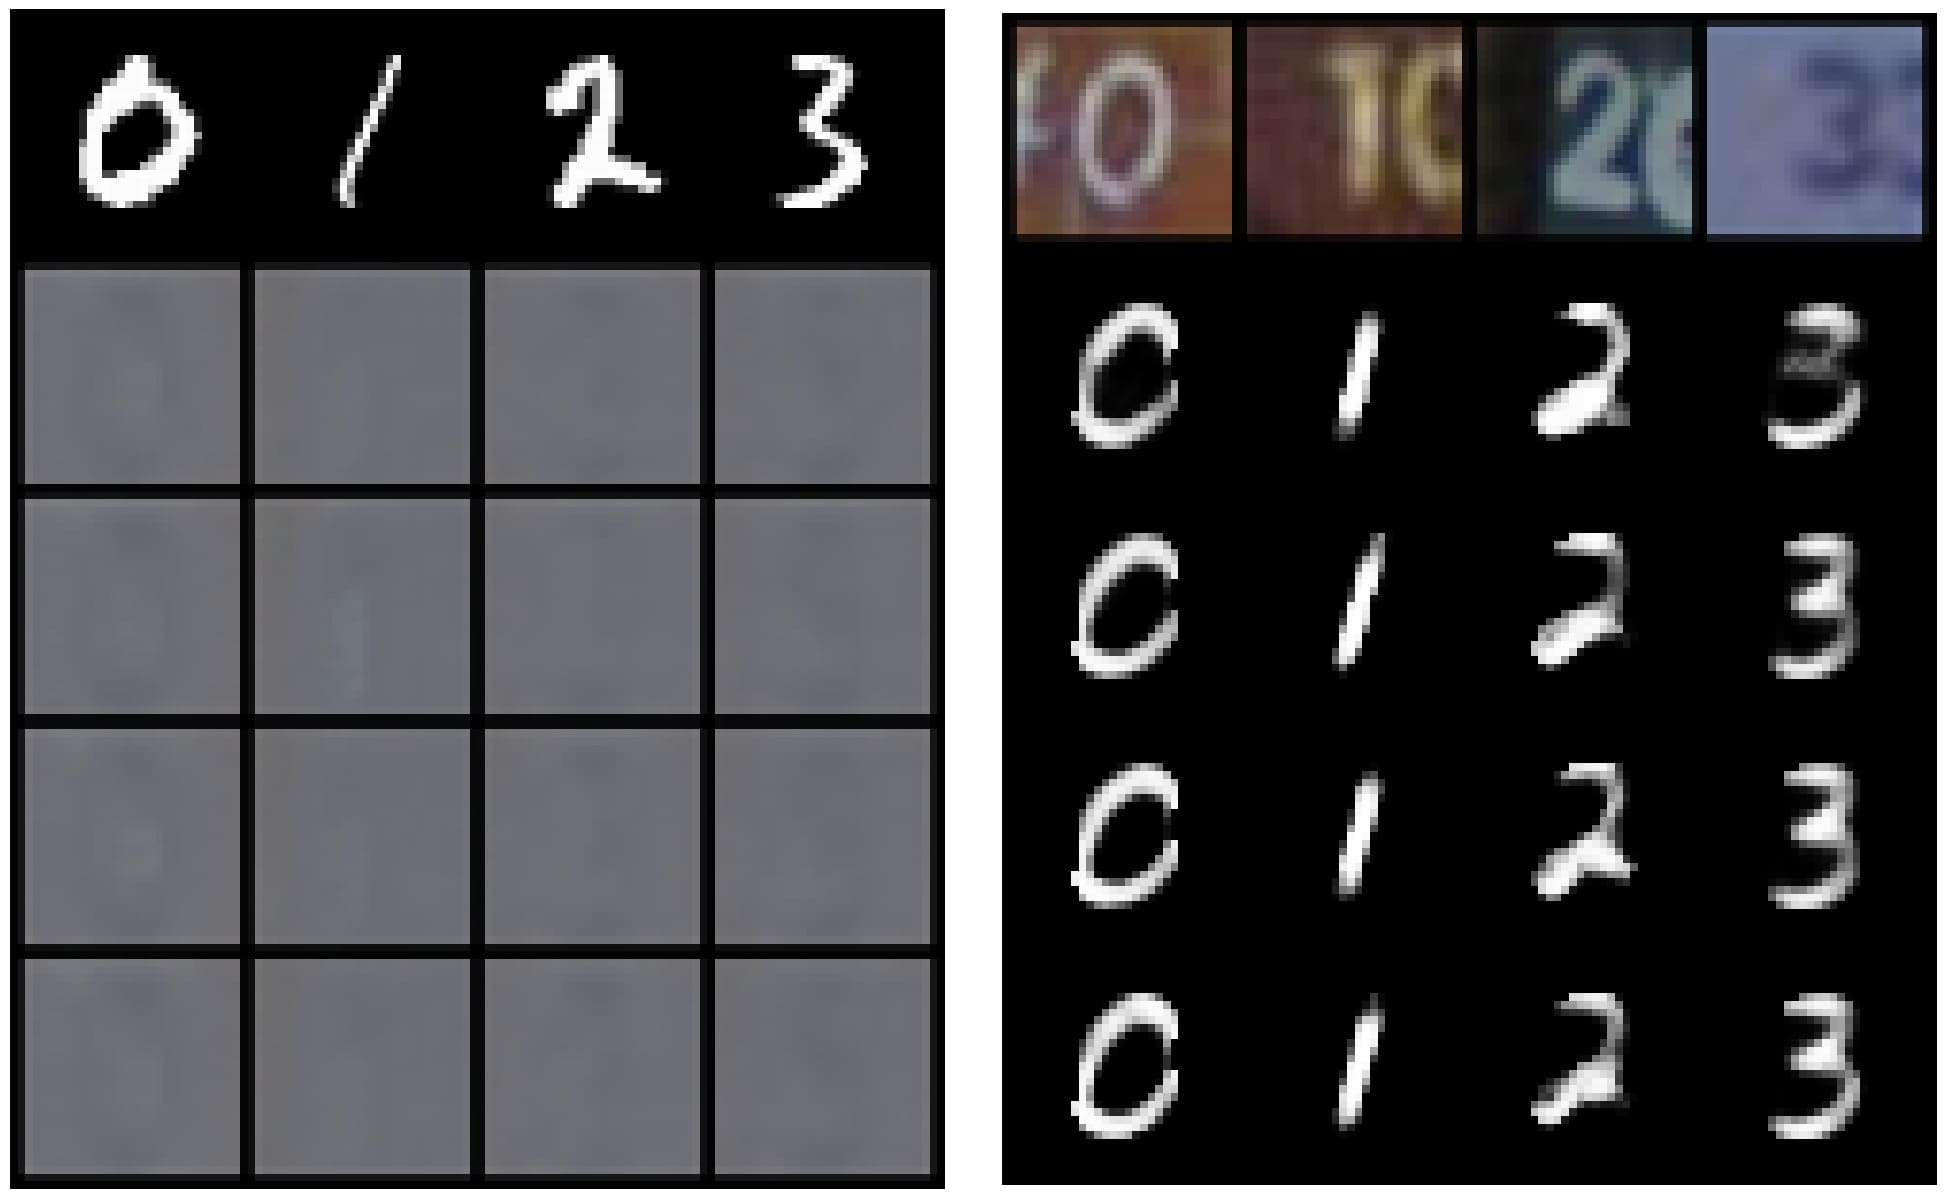
\includegraphics[width=\linewidth]{figures/datasets/ms/smallmmvae_cond_mnist_svhn}
         \caption*{\gls{MMVAE}}
\end{subfigure}
\begin{subfigure}{0.15\textwidth}
         \centering
         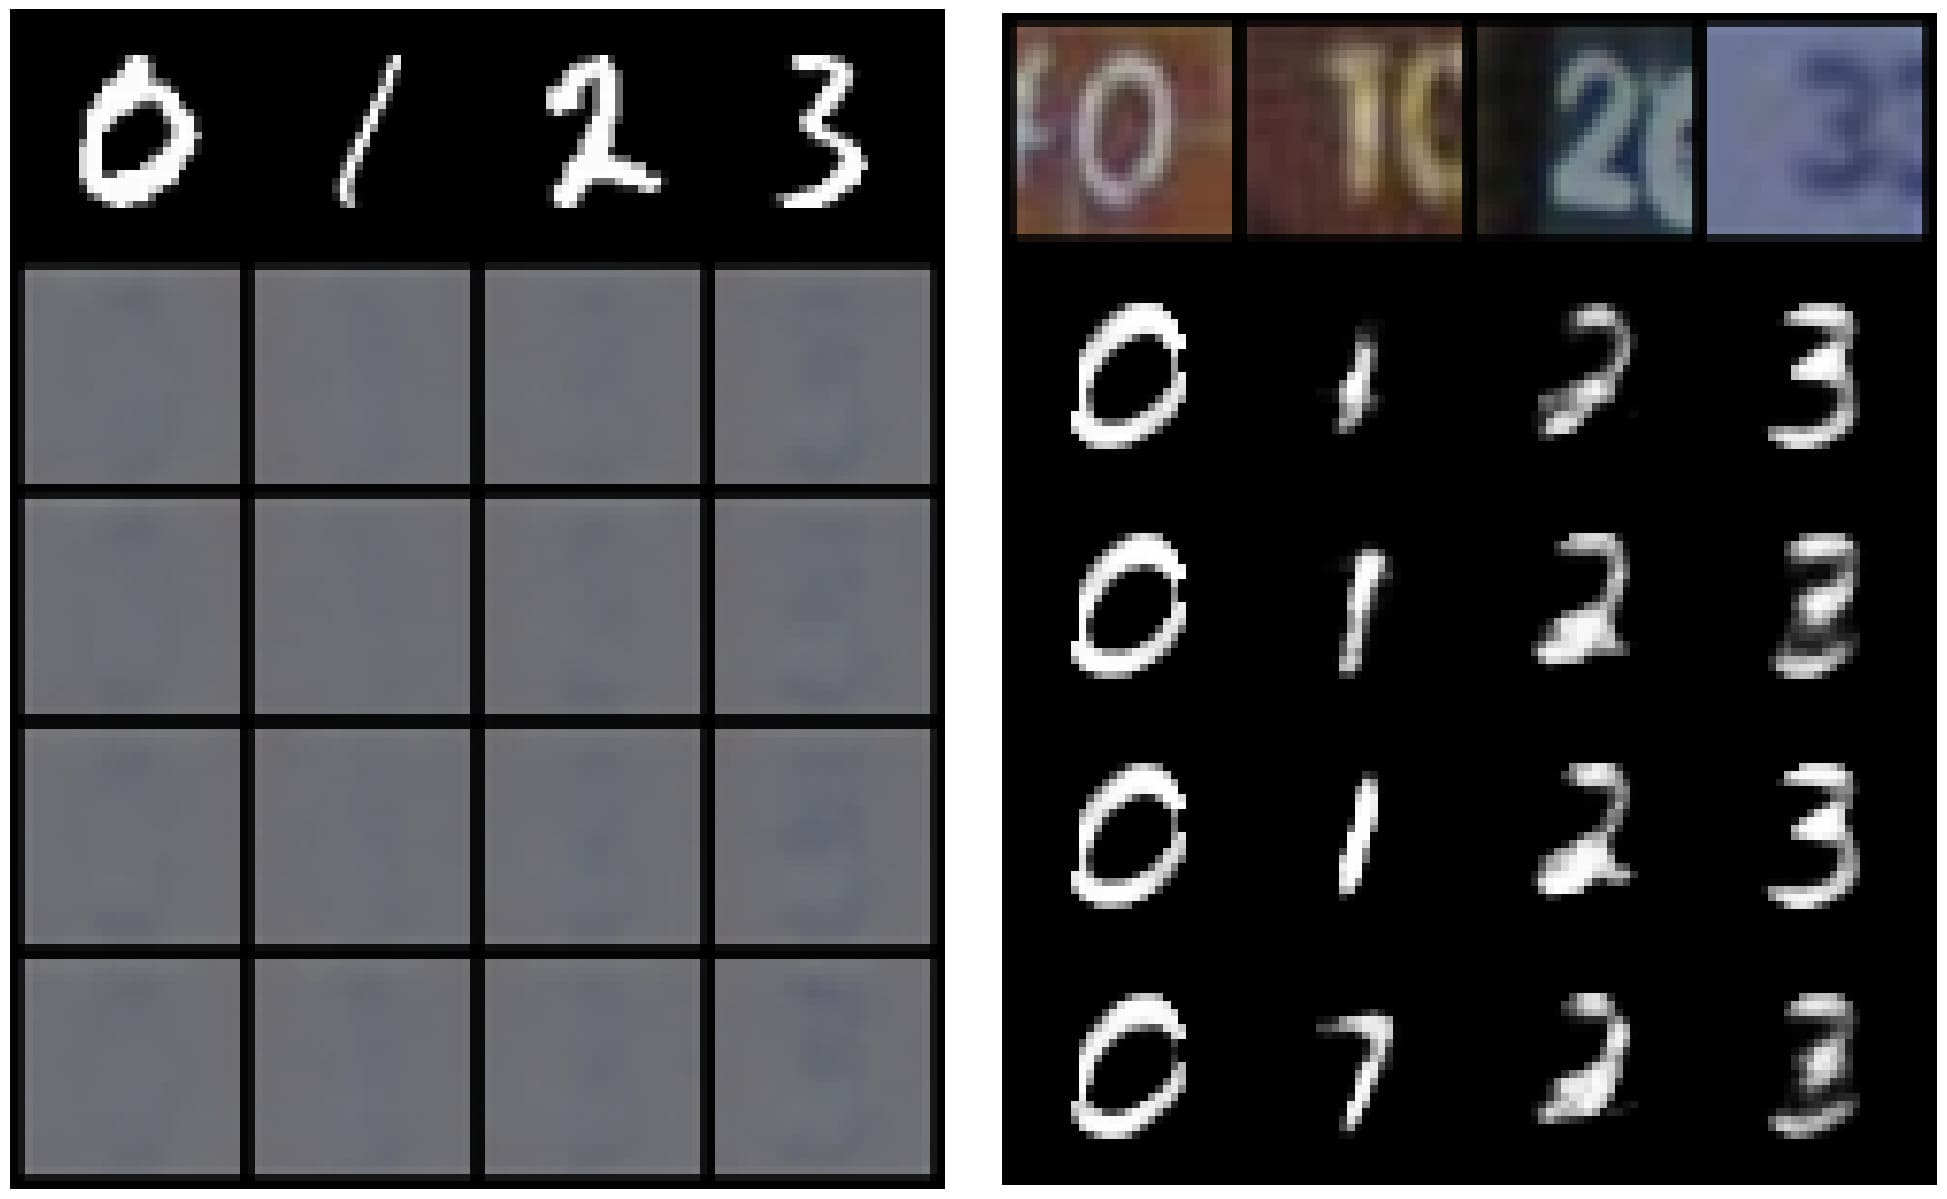
\includegraphics[width=\linewidth]{figures/datasets/ms/smallmopoe_cond_mnist_svhn}
         \caption*{\gls{MOPOE}}
     \end{subfigure}
\begin{subfigure}{0.15\textwidth}
         \centering
         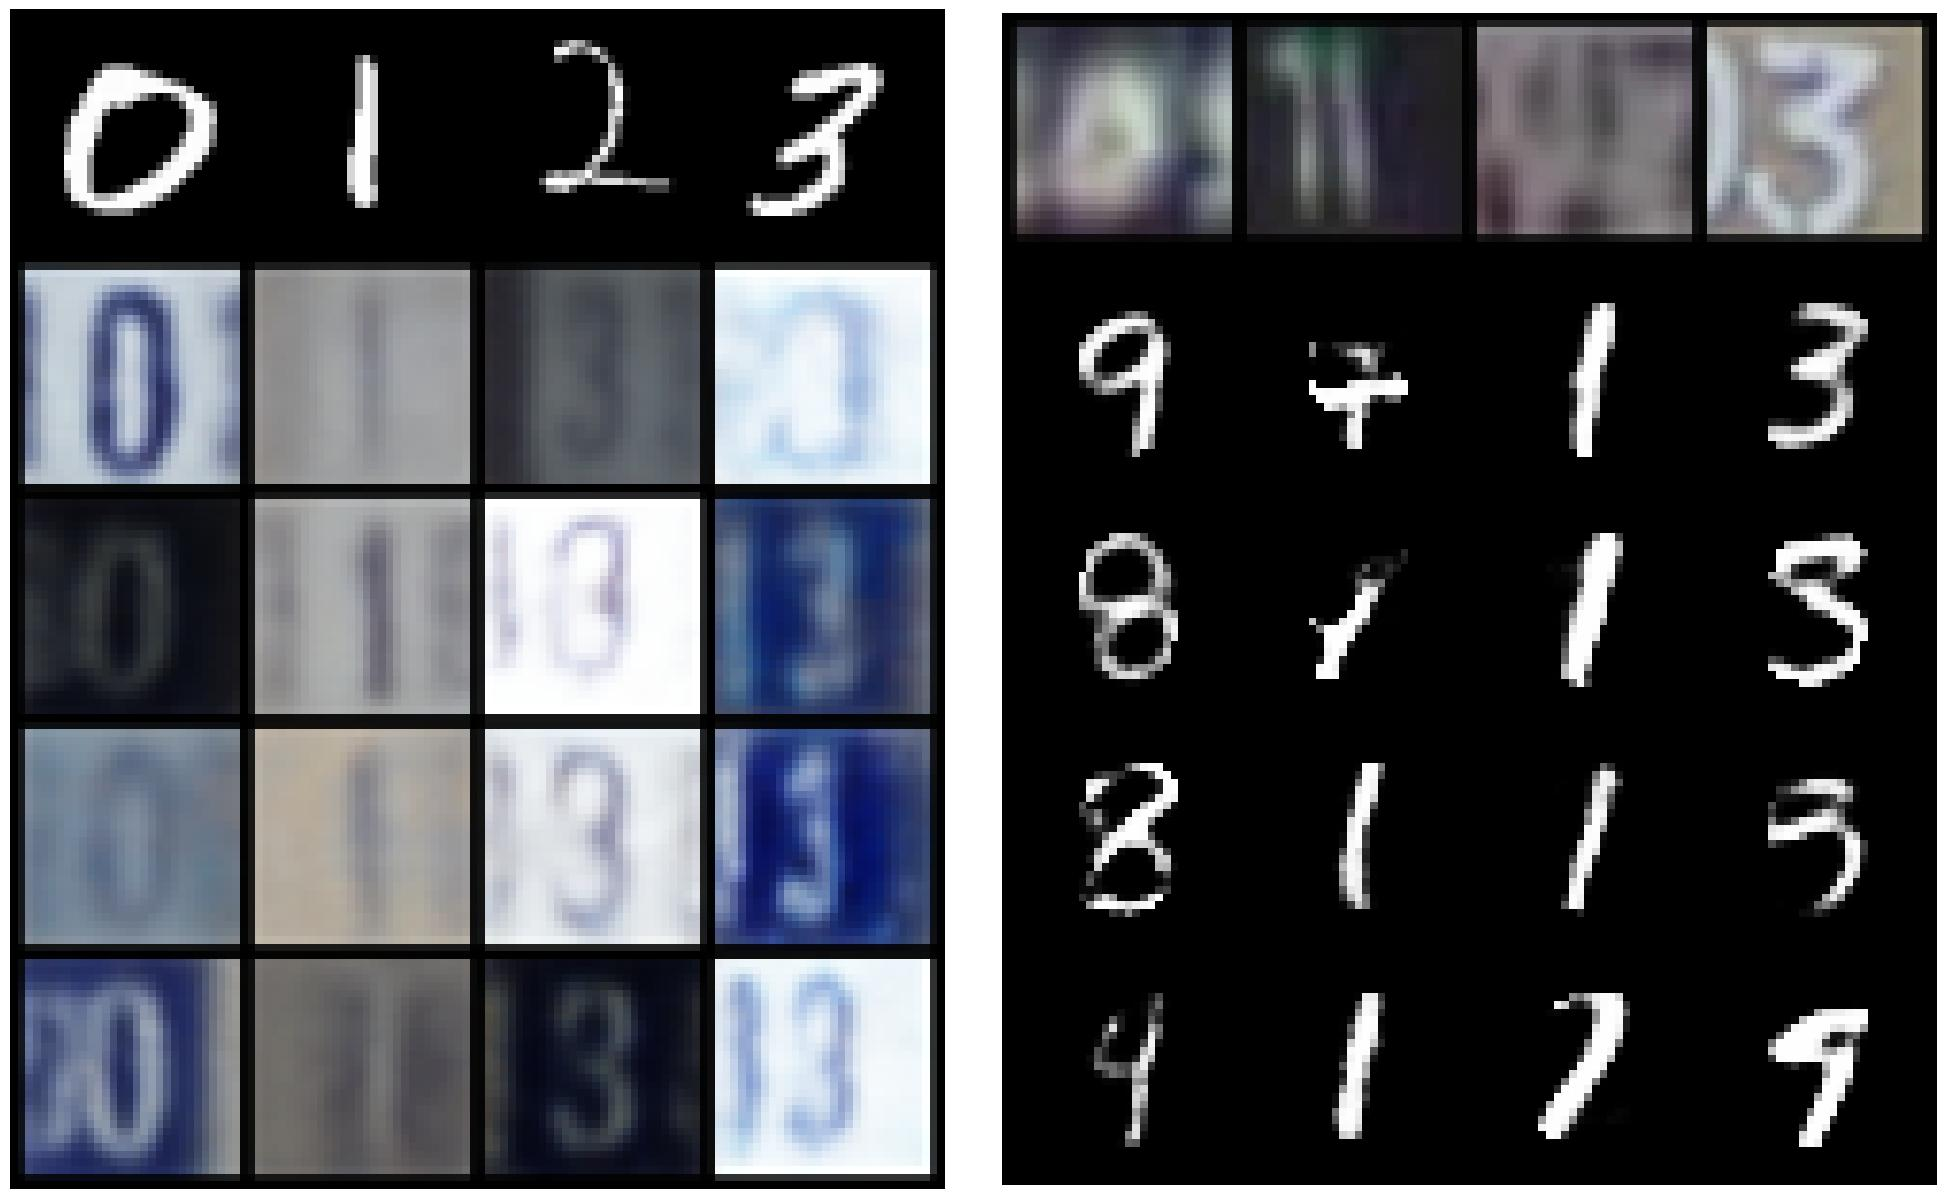
\includegraphics[width=\linewidth]{figures/datasets/ms/small_ms_mmvae+_cond_mnist_svhn.jpg}
    \caption*{\gls{MMVAEplus}(10)}
    \end{subfigure}
\begin{subfigure}{0.15\textwidth}
         \centering
         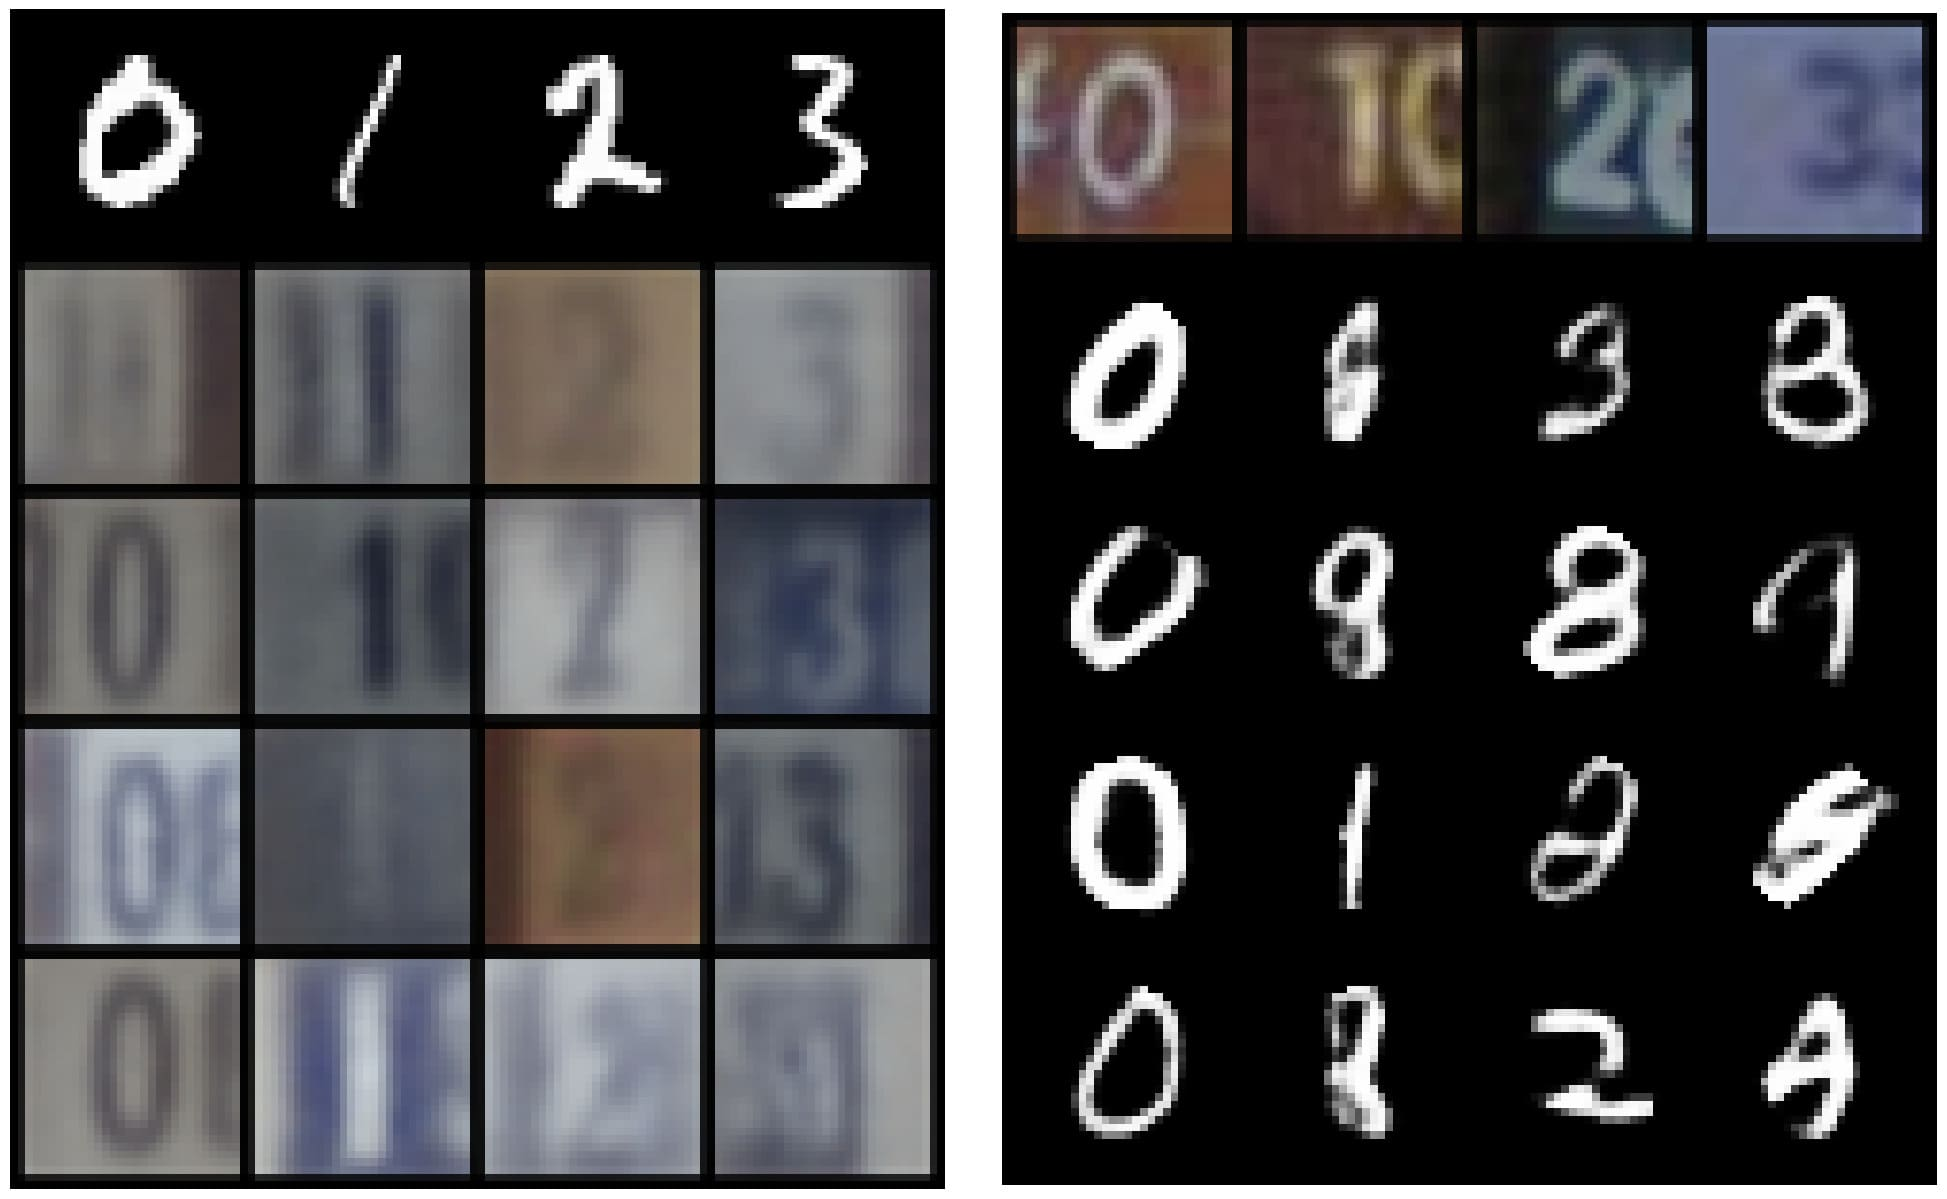
\includegraphics[width=\linewidth]{figures/datasets/ms/smallmvtcae_cond_mnist_svhn}
         \caption*{\gls{MVTCAE}}
\end{subfigure}
  \begin{subfigure}{0.15\textwidth}
         \centering
         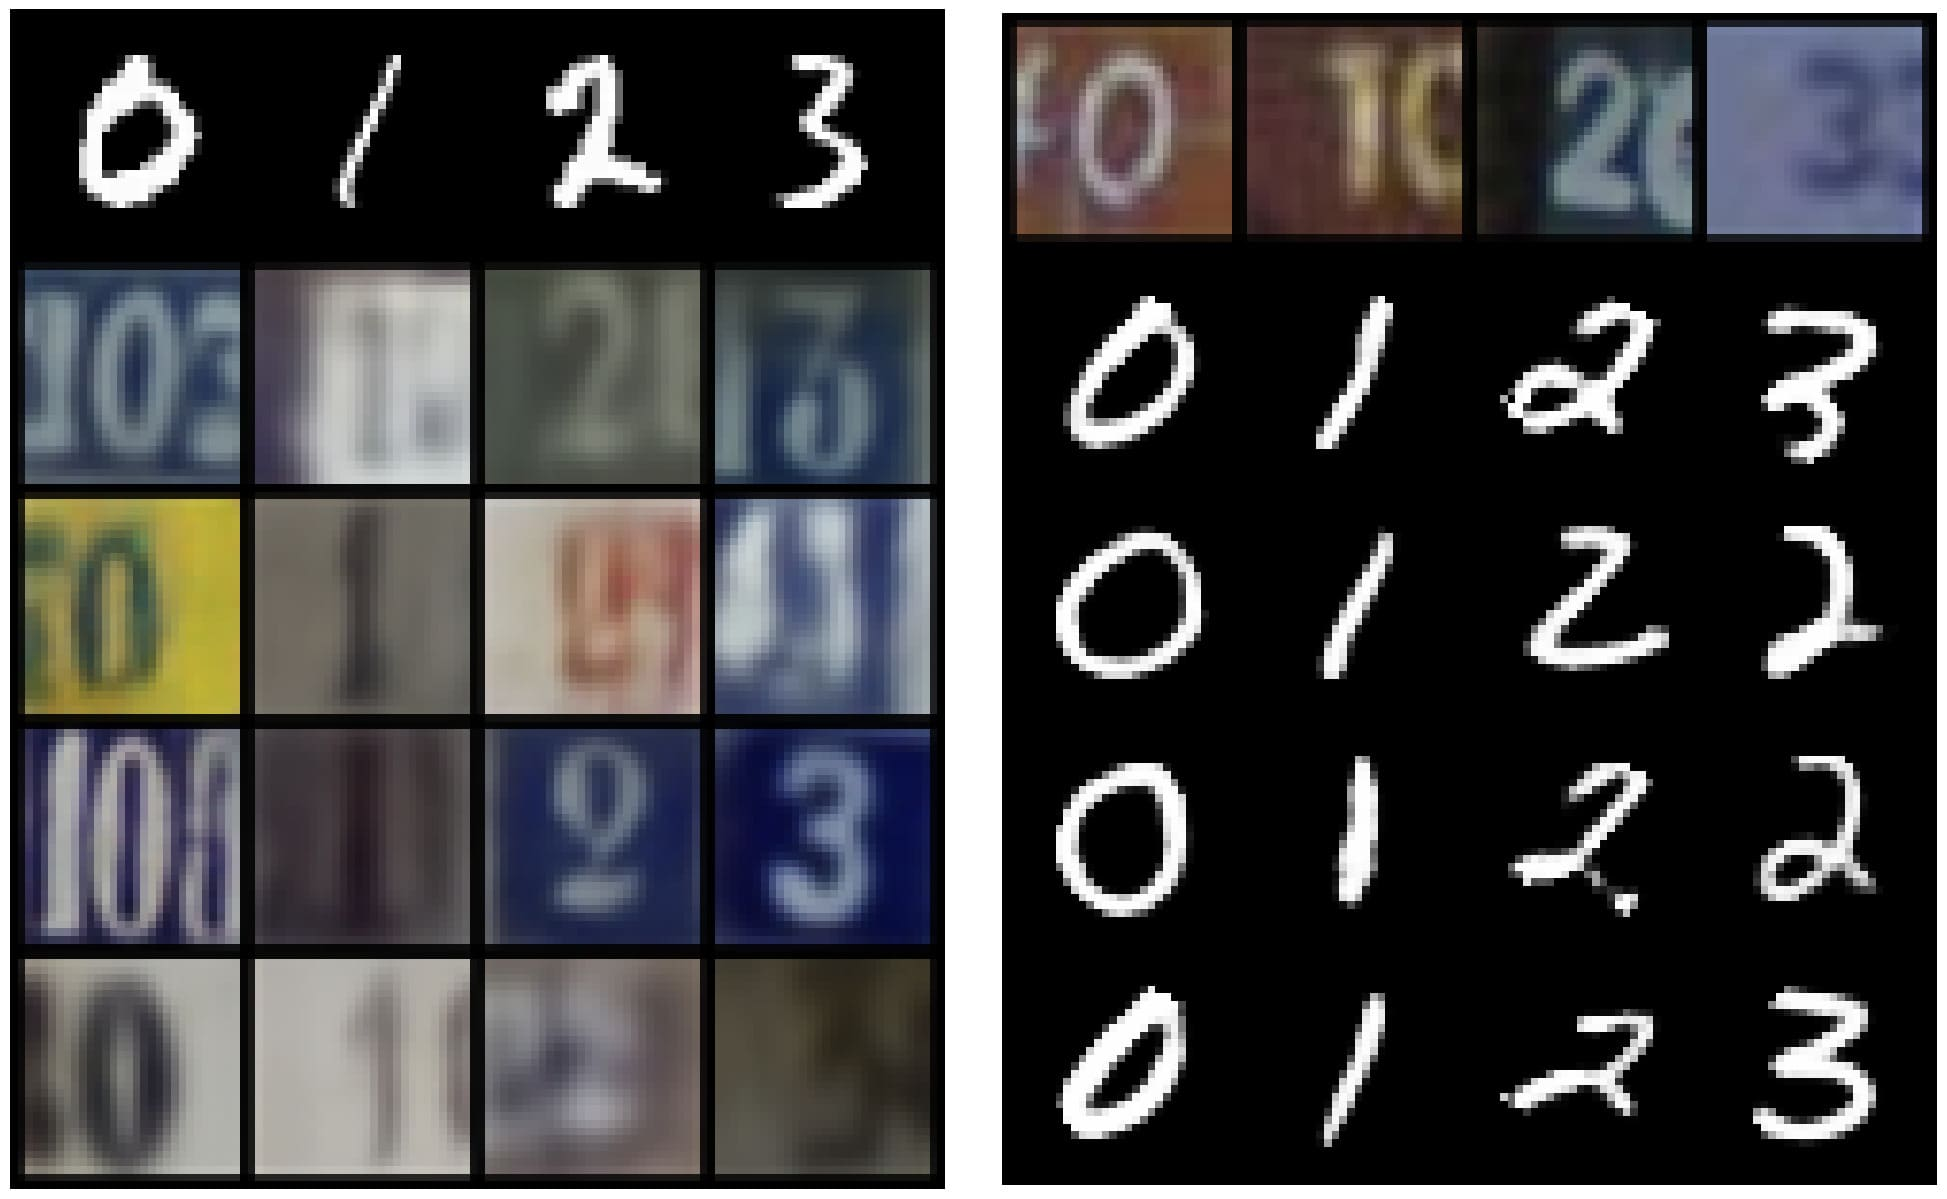
\includegraphics[page=1,width=\linewidth]{figures/datasets/ms/smallMLD_cond_mnist_svhn}
         \caption*{\textbf{\gls{MLD} (ours)}}
     \end{subfigure}
     % \begin{subfigure}{0.15\textwidth}
%          \centering
%          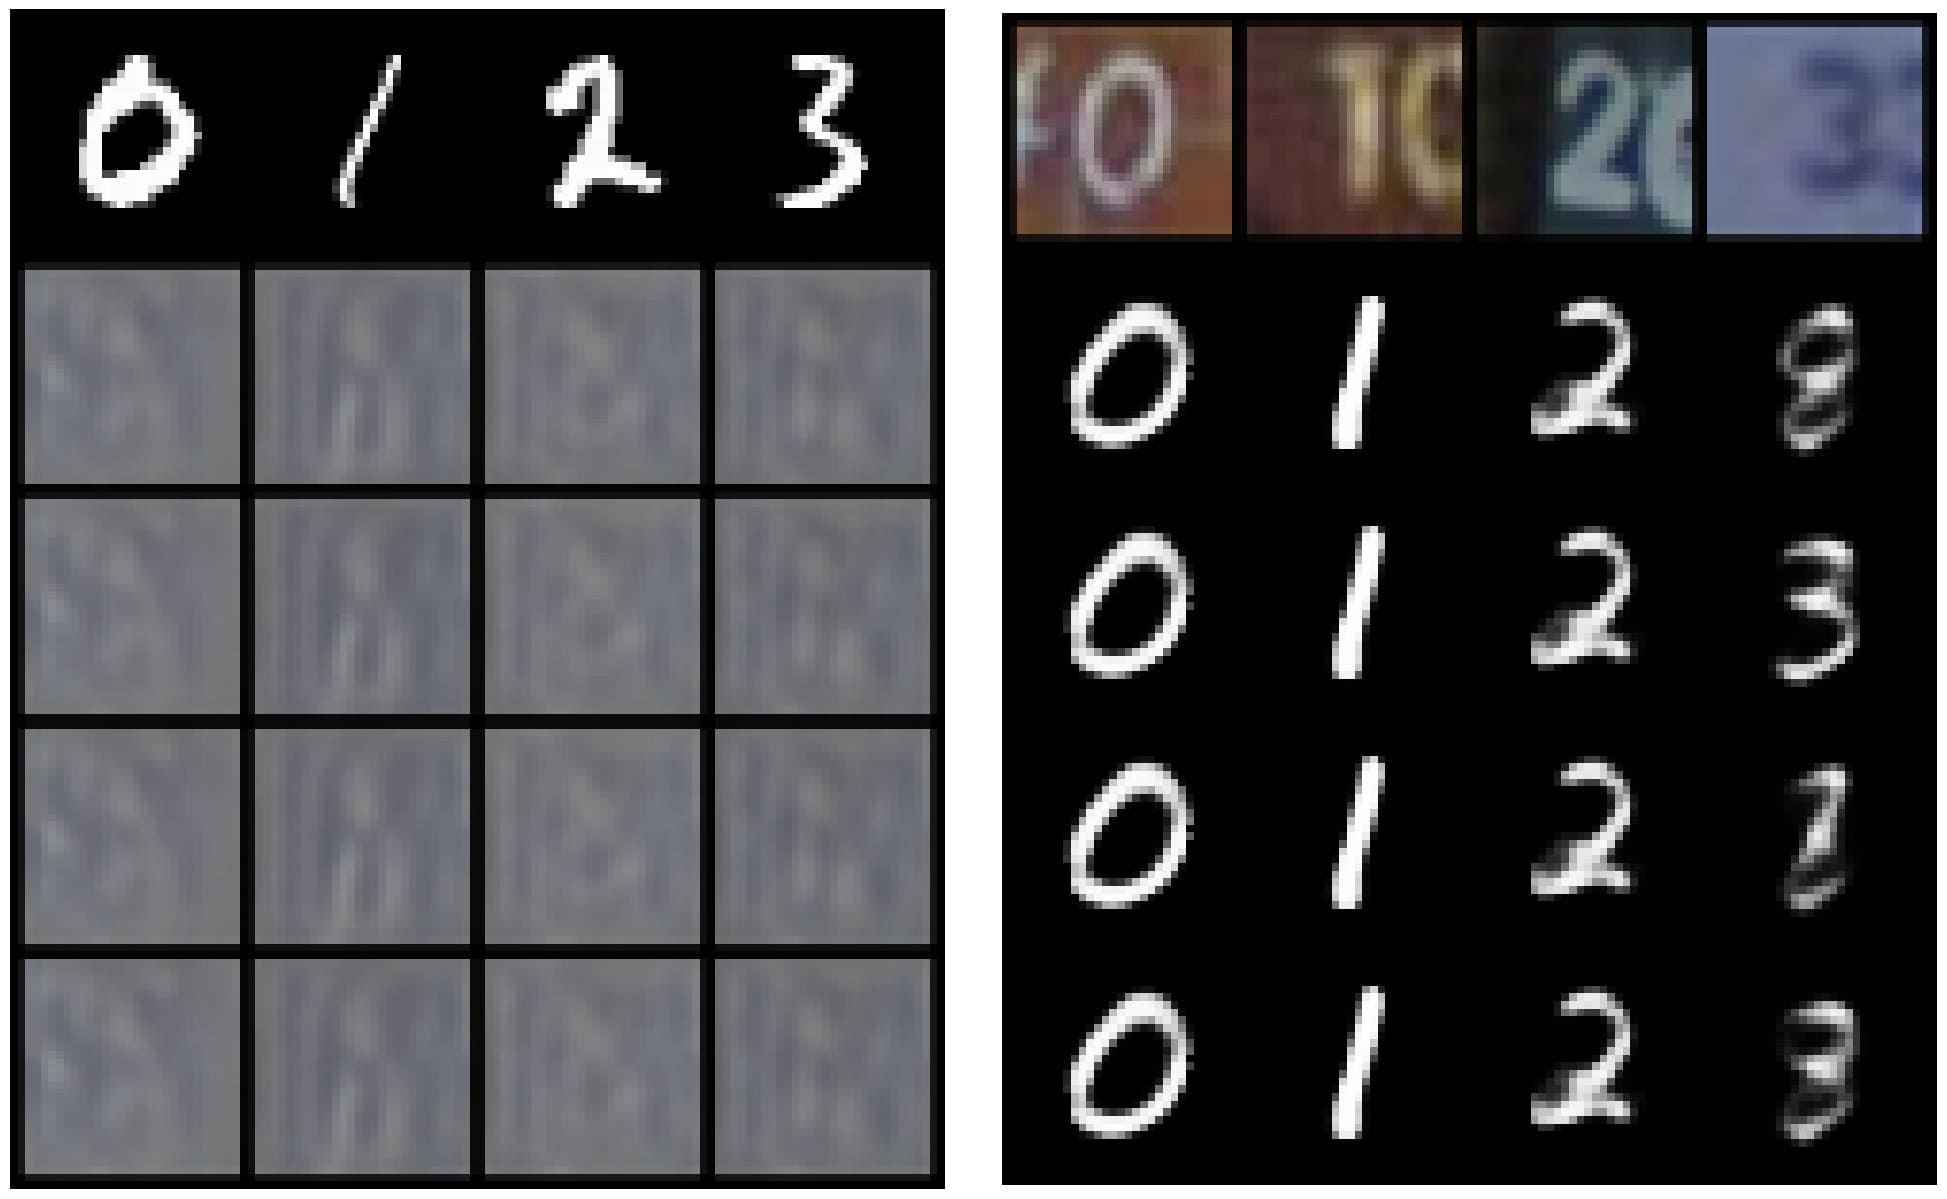
\includegraphics[width=\linewidth]{figures/datasets/ms/smallnexus_cond_mnist_svhn}

%     \caption*{\gls{NEXUS}}
%     \end{subfigure}
\caption{Qualitative results for \textbf{\mnist-\svhn}. For each model we report: \mnist to \svhn conditional generation in the left,   \svhn to \mnist conditional generation in the right.}
        \label{fig:cond_joint_ms}
\end{figure}



The Multi-modal Handwritten Digits data-set (\textbf{\mhd}) \citep{Vasco2022} contains gray-scale digit images, motion trajectory of the hand writing and sounds of the spoken digits. In our experiments, we do not use the label as a forth modality. While digit image and trajectory share a good amount of information, the sound modality contains a lot more of modality specific variation. Consequently, conditional generation involving the sound modality, along with joint generation, are challenging tasks.
Coherency-wise (\Cref{coh:mhd}) \gls{MLD} outperforms all the competitors where the biggest difference is seen in joint and sound to other modalities generation (in the latter task \gls{MVTCAE} performs better than other competitors but is still worse than \gls{MLD}). \gls{MLD} dominates alternatives also in terms of generation quality (\Cref{qua:mhd}). %This is true both for image, sound modalities, for which some \gls{VAE}-based models suffer in producing high quality results, demonstrating the limitation of these methods in handling highly heterogeneous modalities. \gls{MLD}, in the other hand, achieves high generation quality for all modalities, possibly due to the absence of interference thanks to the independent training of its autoencoders.
This is true both for image, sound modalities, for which some \gls{VAE}-based models suffer in producing high quality results, demonstrating the limitation of these methods in handling highly heterogeneous modalities. \gls{MLD}, in the other hand, achieves high generation quality for all modalities, possibly due to the independent training of the autoencoders avoiding interference.



\begin{table}[ht]
\centering
\tiny
\caption{Generation Coherence (\%) for \textbf{\mhd} (Higher is better). Line above refer to the generated modality while the observed modalities subset are presented below.
}  

\begin{tabular}{c|c|ccc|ccc|ccc}
\toprule
\multirow{2}{*}{ Models }  & \multirow{2}{*}{ Joint }  & \multicolumn{3}{c}{I (Image)}  & \multicolumn{3}{c}{T (Trajectory)}  & \multicolumn{3}{c}{S (Sound) } 
\\
\cmidrule{3-11}
    &&  T & S  & T,S  & I & S  & I,S & I & T & I,T \\
    \midrule
    \gls{MVAE} &$37.77$ &
    
    $11.68$ &
    $26.46$ & 
    $ 28.4$ & 
    
    $95.55$  &
    $26.66$ &
     $96.58$ &  
    
    $58.87$ & 
    $10.76$  & 
    $58.16$    \\

     \gls{MMVAE} &    
    $34.78$ &
    
    $\textbf{99.7}$ &
    $69.69 $ & 
    $ 84.74$ & 
    $\underline{99.3}$  &
    $85.46 $  & 
    $92.39$ & 
    $49.95$ & 
    $50.14$  & 
    $50.17$   \\
   
     \gls{MOPOE}   &   $48.84$ &
    $\underline{99.64}$ & $68.67$ & $ \underline{99.69}$ & 
    $99.28$  & $\underline{87.42}$  & $99.35$ &  
    $50.73$ & $51.5$  & $56.97$   \\

     \gls{NEXUS} &  $26.56$ &
    $94.58$ & $\underline{83.1}$ & $ 95.27$ & 
    $88.51$  & $76.82$  & $93.27$ &  
    $70.06$ & $75.84$  & $89.48$ 
    \\
      \gls{MVTCAE} &  $42.28$ 
     &
    $99.54$ & $72.05$ & $ 99.63$ & 
    $99.22$  & $72.03$  & $\underline{99.39}$ &  
    $\underline{92.58}$ & $\underline{93.07}$  & $\underline{94.78}$  \\

 
      \gls{MMVAEplus} &  $41.67$ 
     &
    $98.05$ & $84.16$ & $ 91.88_{\pm }$ & 
    $97.47$  & $81.16$  & $89.31$ &  
    $64.34$ & 
    $65.42$  &
    $64.88$  \\

   \gls{MMVAEplus}(k=10) &  $42.60$ 
     &
    $99.44$ & $\textbf{89.75}$ & $ 94.7$ & 
    $99.44$  
    & $\textbf{89.58}$  & $95.01$ &  
    $87.15$ & 
    $87.99$  &
    $87.57$  
    
\\
    \midrule
\textbf{\gls{MLD} (ours)} &  
    $\textbf{98.34}$ &
    $99.45$ &
    $\underline{88.91}$ & 
    $ \textbf{99.88}$ & 
    
    $\textbf{99.58}$  & 
    $\underline{88.92}$  & 
    $\textbf{99.91}$ &  
    
    $\textbf{97.63}$ & 
    $\textbf{97.7}$ 
    & $\textbf{98.01}$  \\
    \bottomrule


   
\end{tabular}

 \label{coh:mhd}

\end{table}





\begin{table}[h]
\centering
\tiny
\caption{Generation quality for \textbf{\mhd} in terms of \gls{FMD} for image and trajectory modalities and \gls{FAD} for the sound modality (Lower is better).}
\resizebox{0.9\textwidth}{!}{\begin{tabular}{c|cccc|cccc|cccc}
\toprule
\multirow{2}{*}{ Models }  & \multicolumn{4}{c}{I (Image)}  & \multicolumn{4}{c}{T (Trajectory)}  & \multicolumn{4}{c}{S (Sound) } 
\\
\cmidrule{2-13}
   & Joint & T & S  & T,S    &  Joint  & I & S  & I,S  & Joint &  I & T & I,T   \\
    \midrule
    \gls{MVAE} &
    $\underline{94.9}$  
    & $93.73$ &
    $92.55$  &
    $91.08$  &
    
    
    $39.51$   &
    $20.42$ &
    $38.77$  &
    $19.25$  &
    

     
    $14.14$ &
  $\underline{14.13}$ &
    $14.08$  &
    $14.17$   

    \\
  \gls{MMVAE} 
  &$224.01$   
  &  $22.6$ &
    $789.12$  &
    $170.41$  &
    
    
    $16.52$   &
    $\textbf{0.5}$ &
    $30.39$  &
    $6.07$  &
    

    
     $22.8$  &
    $22.61$ &
    $23.72$  &
    $23.01$  
     

\\
    \gls{MOPOE} & 
    $147.81$   & 
    $16.29$ &
    $838.38$  &
    $15.89$  &
    
    
$\underline{13.92}$   & 
$\underline{0.52}$ &
    $33.38$  &
    $\textbf{0.53}$  &
    
     
    $18.53$ &
    $24.11$ &
    $24.1$  &
    $23.93$ 
    
    \\
    \gls{NEXUS} &   
    $281.76$   &     
    $116.65$ &
    $282.34$  &
    $117.24$  &
    
    
    $18.59$   &
    $6.67$ &
    $33.01$  &
    $7.54$  &
    
    
    $\underline{13.99}$ &
    $19.52$ &
    $18.71$  &
    $16.3$    

    \\
    \gls{MVTCAE} &
    $121.85$  &   $\underline{5.34}$ &
    $\underline{54.57}$  &
    $\underline{3.16}$  &
     
    $19.49$   &
    $0.62$ &
    $\underline{13.65}$  &
    $0.75$  &
    
    
    $15.88$   &
    $14.22$ &
    $\underline{14.02}$  &
    $\underline{13.96}$  
    \\

    
   \gls{MMVAEplus} &    
   
   $97.19$   &  
   $2.80$ &
    $128.56$  &
    $ 114.3$  &
 

        $22.37$   & 
    $1.21$ &
    $21.74$  &
    $15.2$  &


        $16.12$   &
        $17.31$ &
    $17.92$  &
    $17.56$
    
    \\

     \gls{MMVAEplus}(K=10) &    
   
   $85.98$   &  
   $1.83$ &
    $70.72$  &
    $62.43$  &
 

        $21.10$   & 
    $1.38$ &
    $8.52$  &
    $7.22$  &


   $14.58$   &  
   $14.33$ &
    $14.34$  &
    $14.32$  
    \\
    \midrule
    \gls{MLD} 
    &   
    $\textbf{7.98}$ &
    $\textbf{1.7}$ &
    $\textbf{4.54}$ & 
    $\textbf{1.84}$  &
    
    
    $\textbf{3.18}$ 
      & $0.83$ 
     & $\textbf{2.07}$ 
       & $\underline{0.6}$ 
       
       
       & $ \textbf{2.39} $
        & $\textbf{2.31}$ 
     & $\textbf{2.33}$ 
       & $\textbf{	2.29}$ 
       
       \\

    \bottomrule
   
\end{tabular}
}


 \label{qua:mhd}

\end{table}





The \textbf{\polymnist} data-set \citep{sutter2021generalized} consists of 5 modalities synthetically generated by using \mnist digits and varying the background images. The homogeneous nature of the modalities is expected to mitigate gradient conflict issues in \gls{VAE}-based models, and consequently reduce modality collapse. However, \gls{MLD} still outperforms all alternatives, as shown \Cref{fig:res_mmnist}. Concerning generation coherence, \gls{MLD} achieves the best performance in all cases with the single exception of a single observed modality. On the qualitative performance side, not only \gls{MLD} is superior to alternatives, but its results are stable when more modalities are considered, a capability that not all competitors share. 

\begin{figure} [h]
\centering
\begin{subfigure}{0.24\textwidth}
\centering
     \begin{subfigure}{1\textwidth}
         \centering
         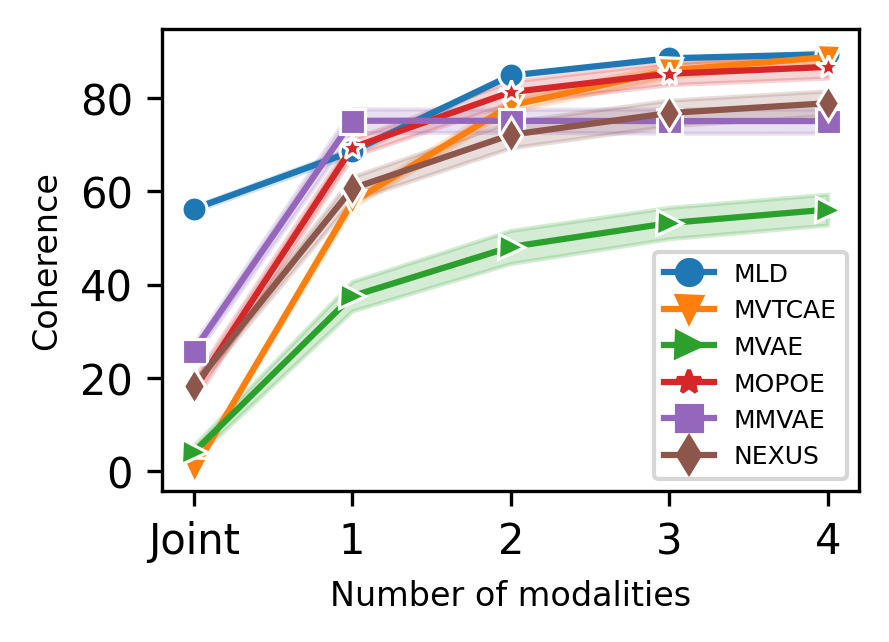
\includegraphics[page=1,width=\linewidth]{figures/datasets/mmnist/quant/bsline_mmnist_plot_coh_avg}
   
     \end{subfigure}
     
     \begin{subfigure}{1\textwidth}
         \centering
         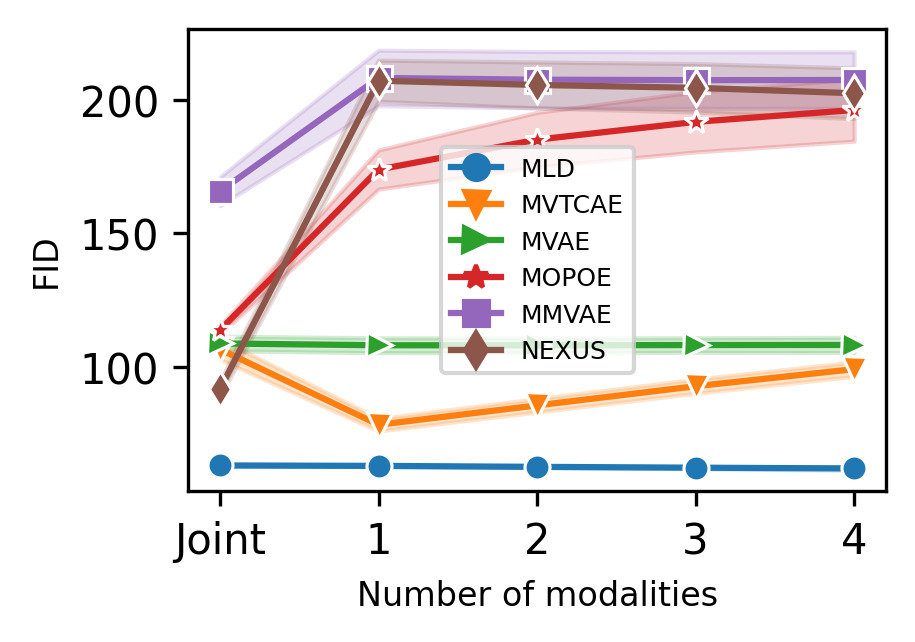
\includegraphics[width=\linewidth]{figures/datasets/mmnist/quant/bsline_mmnist_plot_fid_avg}
   
     \end{subfigure}

\label{mmnist_quantitavie}
     \end{subfigure}
\begin{subfigure}{0.73\textwidth}
     \centering
     \begin{subfigure}{0.25\textwidth}
         \centering
         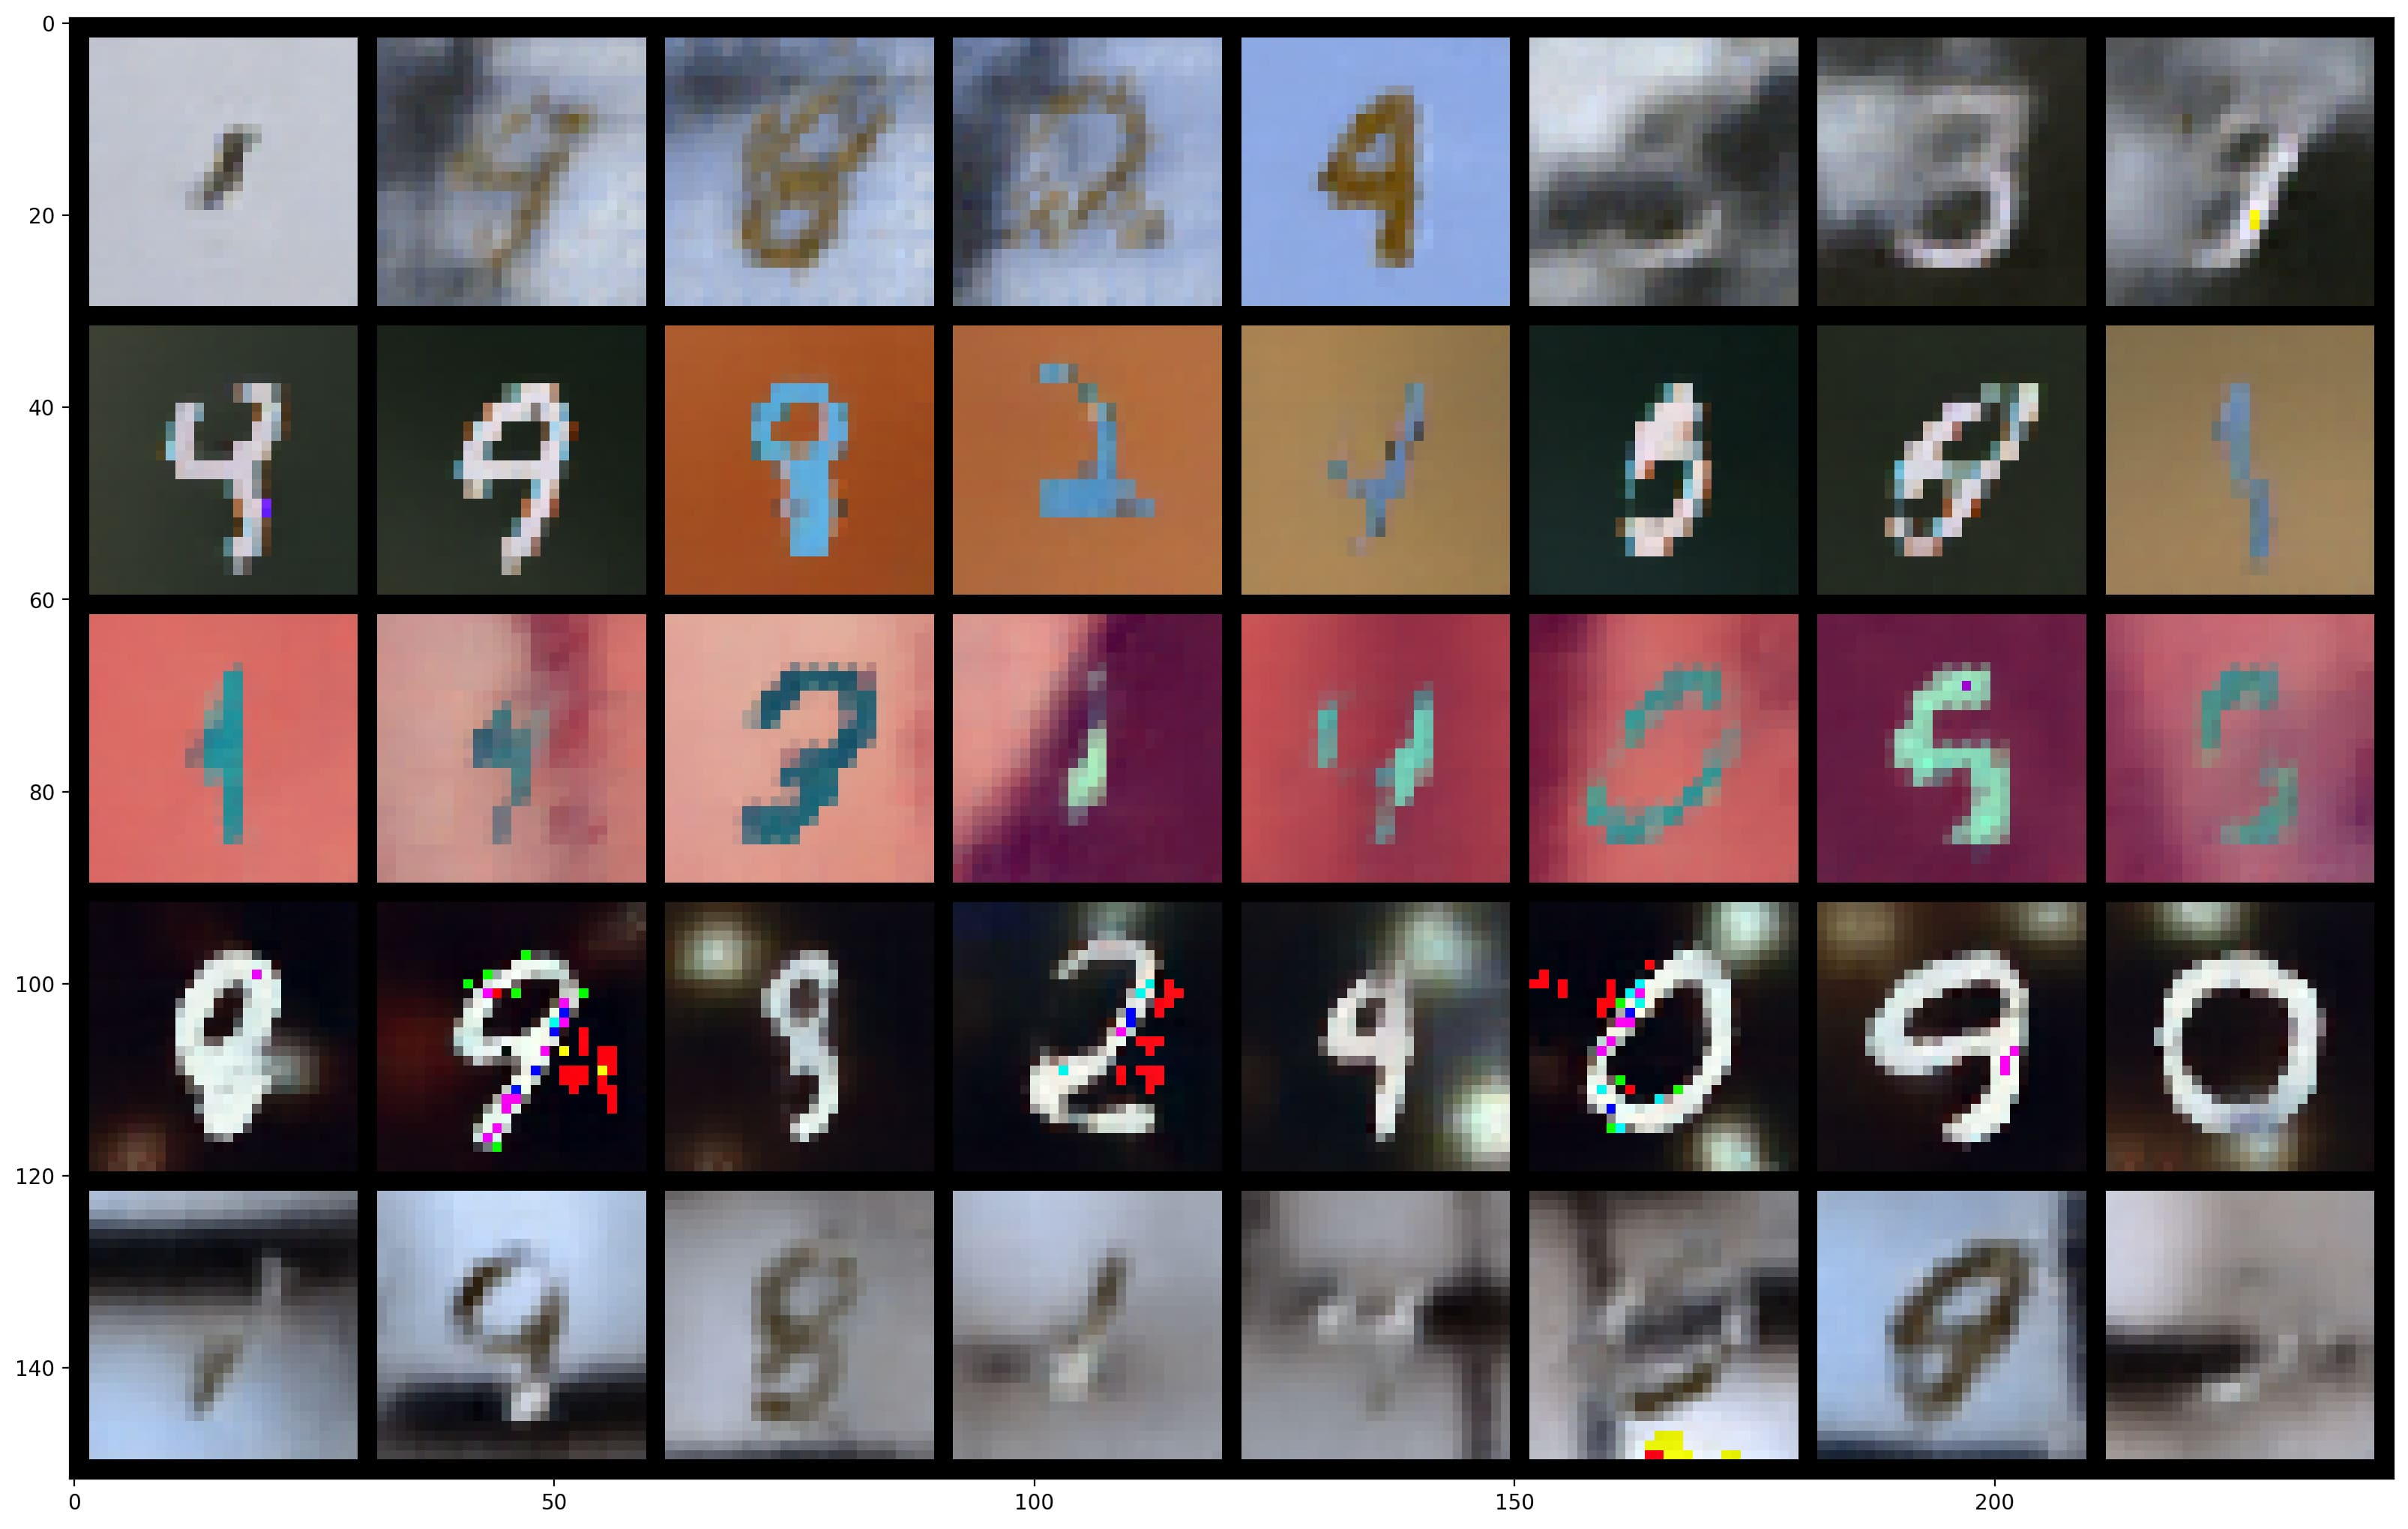
\includegraphics[width=\linewidth]{figures/datasets/mmnist/quali/mvae_sampling}
         \caption*{\gls{MVAE}}
         
     \end{subfigure}
     \begin{subfigure}{0.25\textwidth}
         \centering
         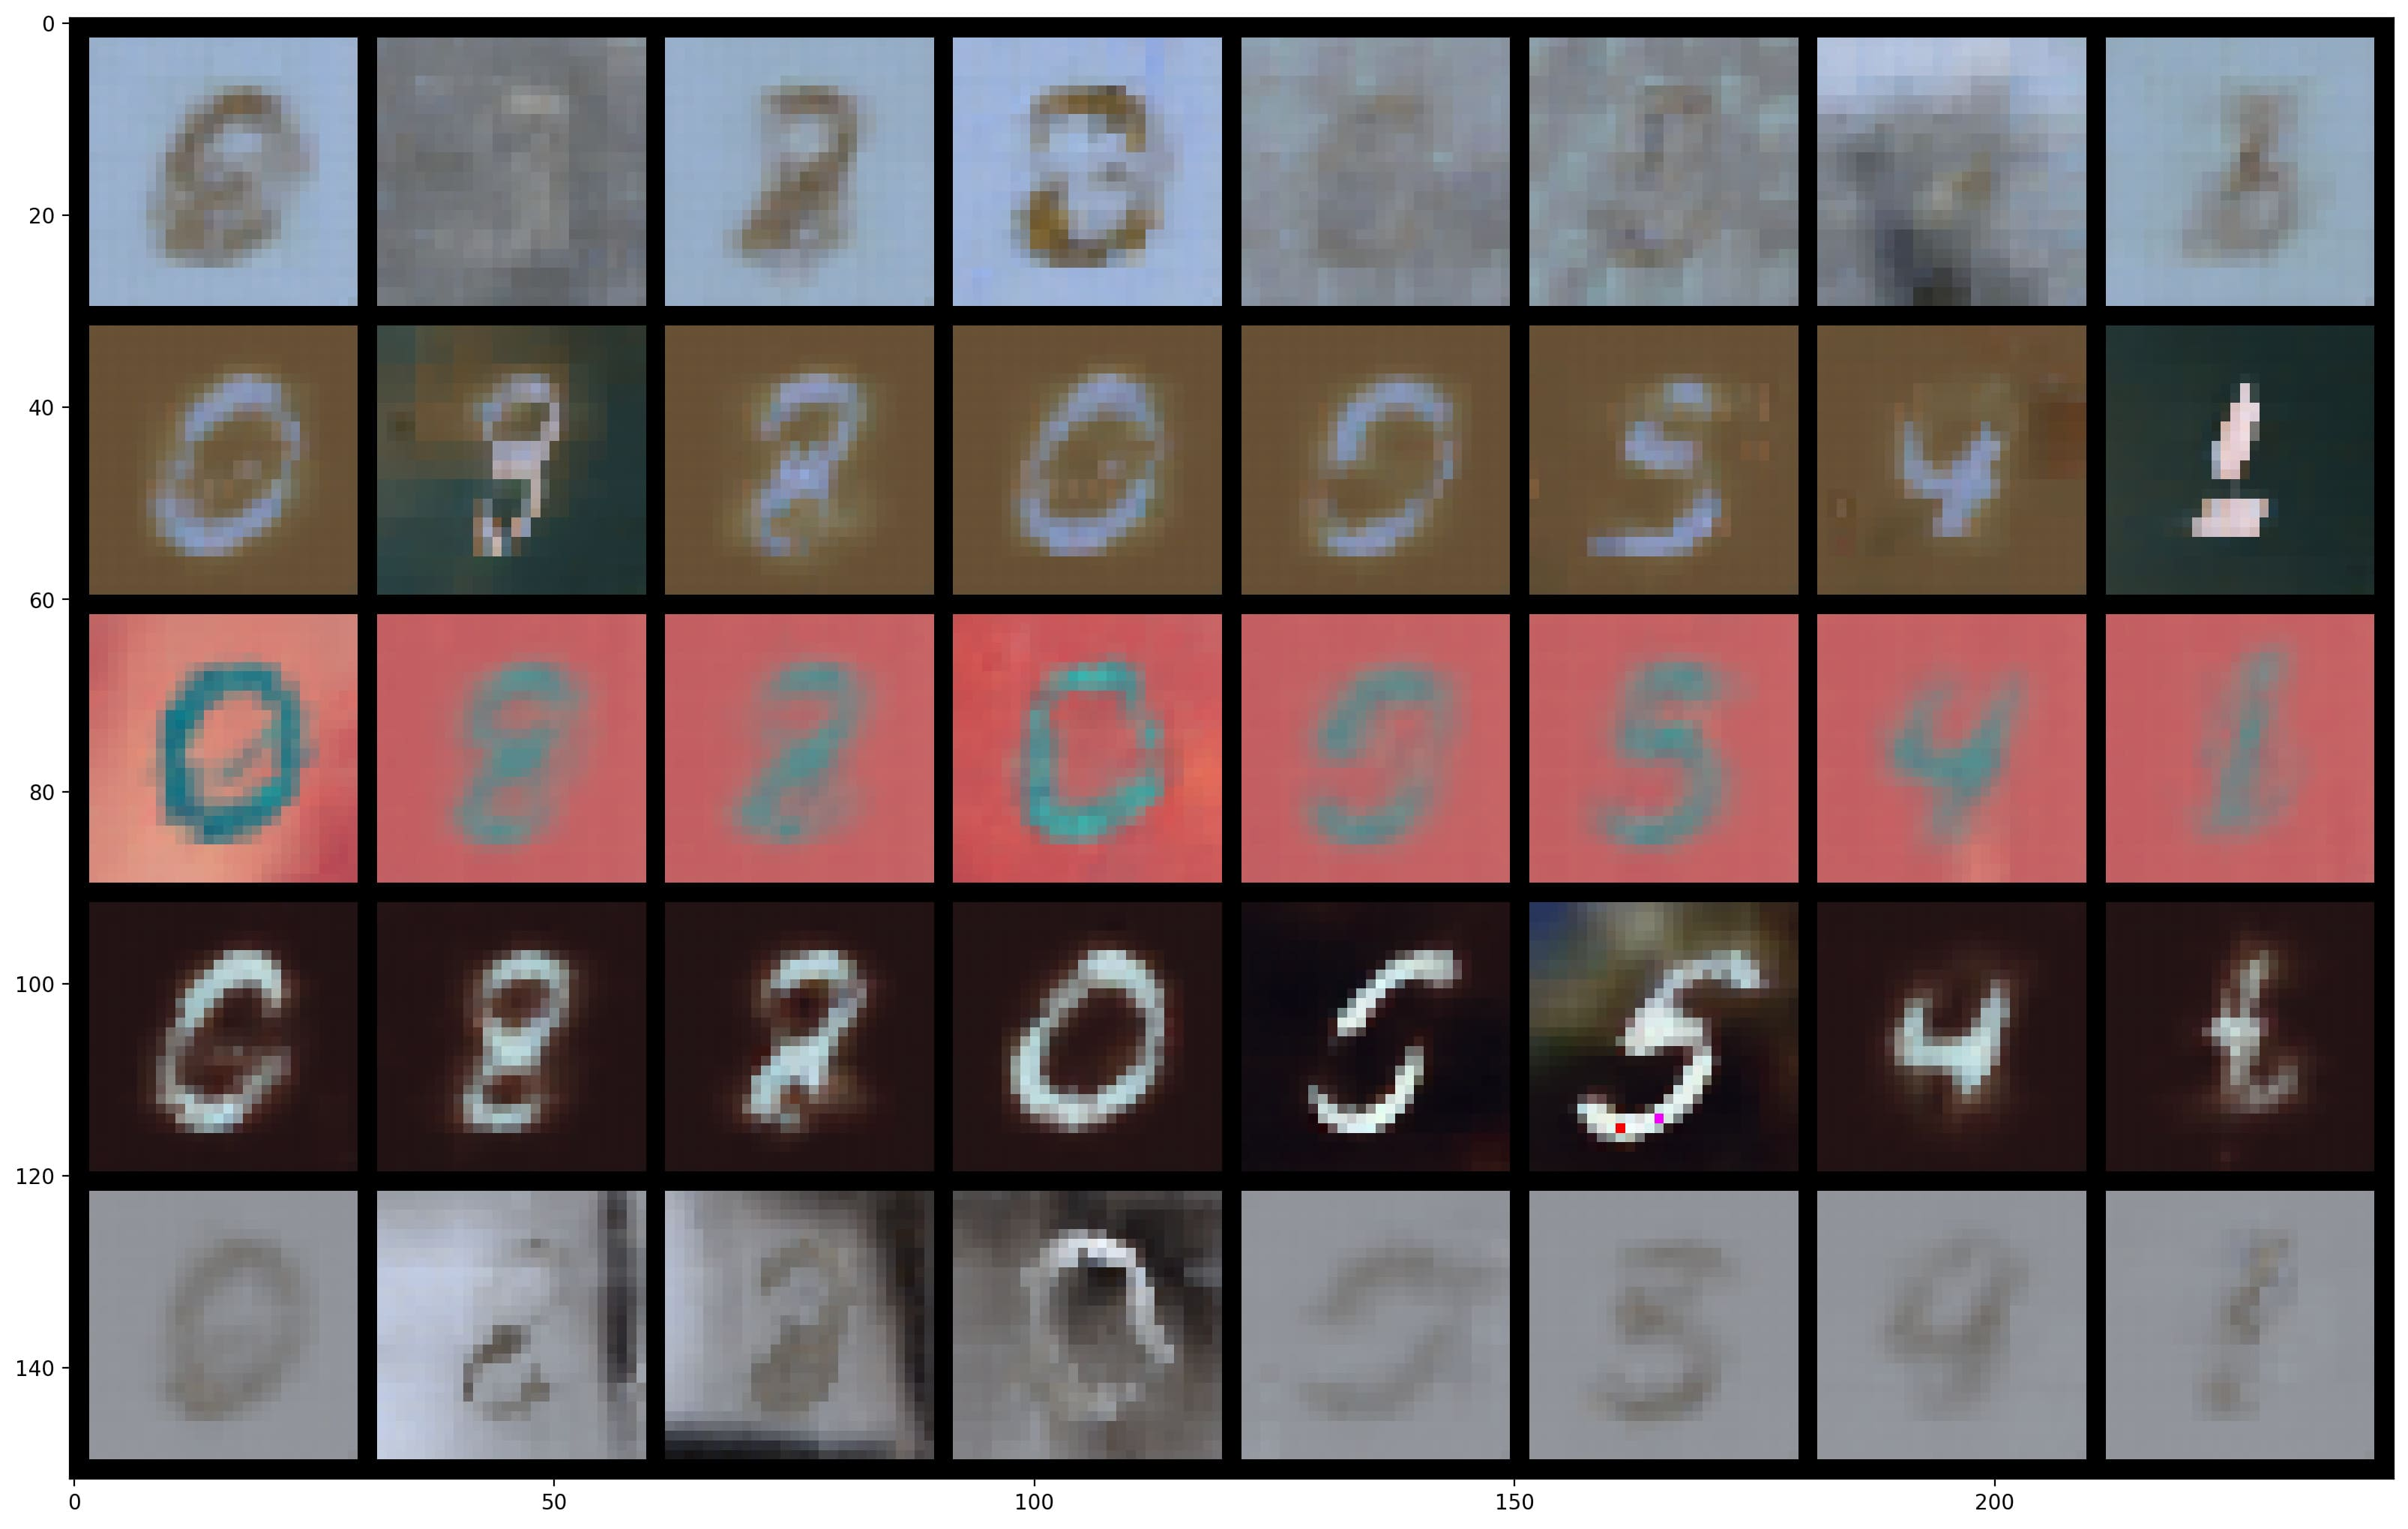
\includegraphics[width=\linewidth]{figures/datasets/mmnist/quali/mmvae_sampling}
         \caption*{\gls{MMVAE}}
      
     \end{subfigure}
       \begin{subfigure}{0.25\textwidth}
         \centering
         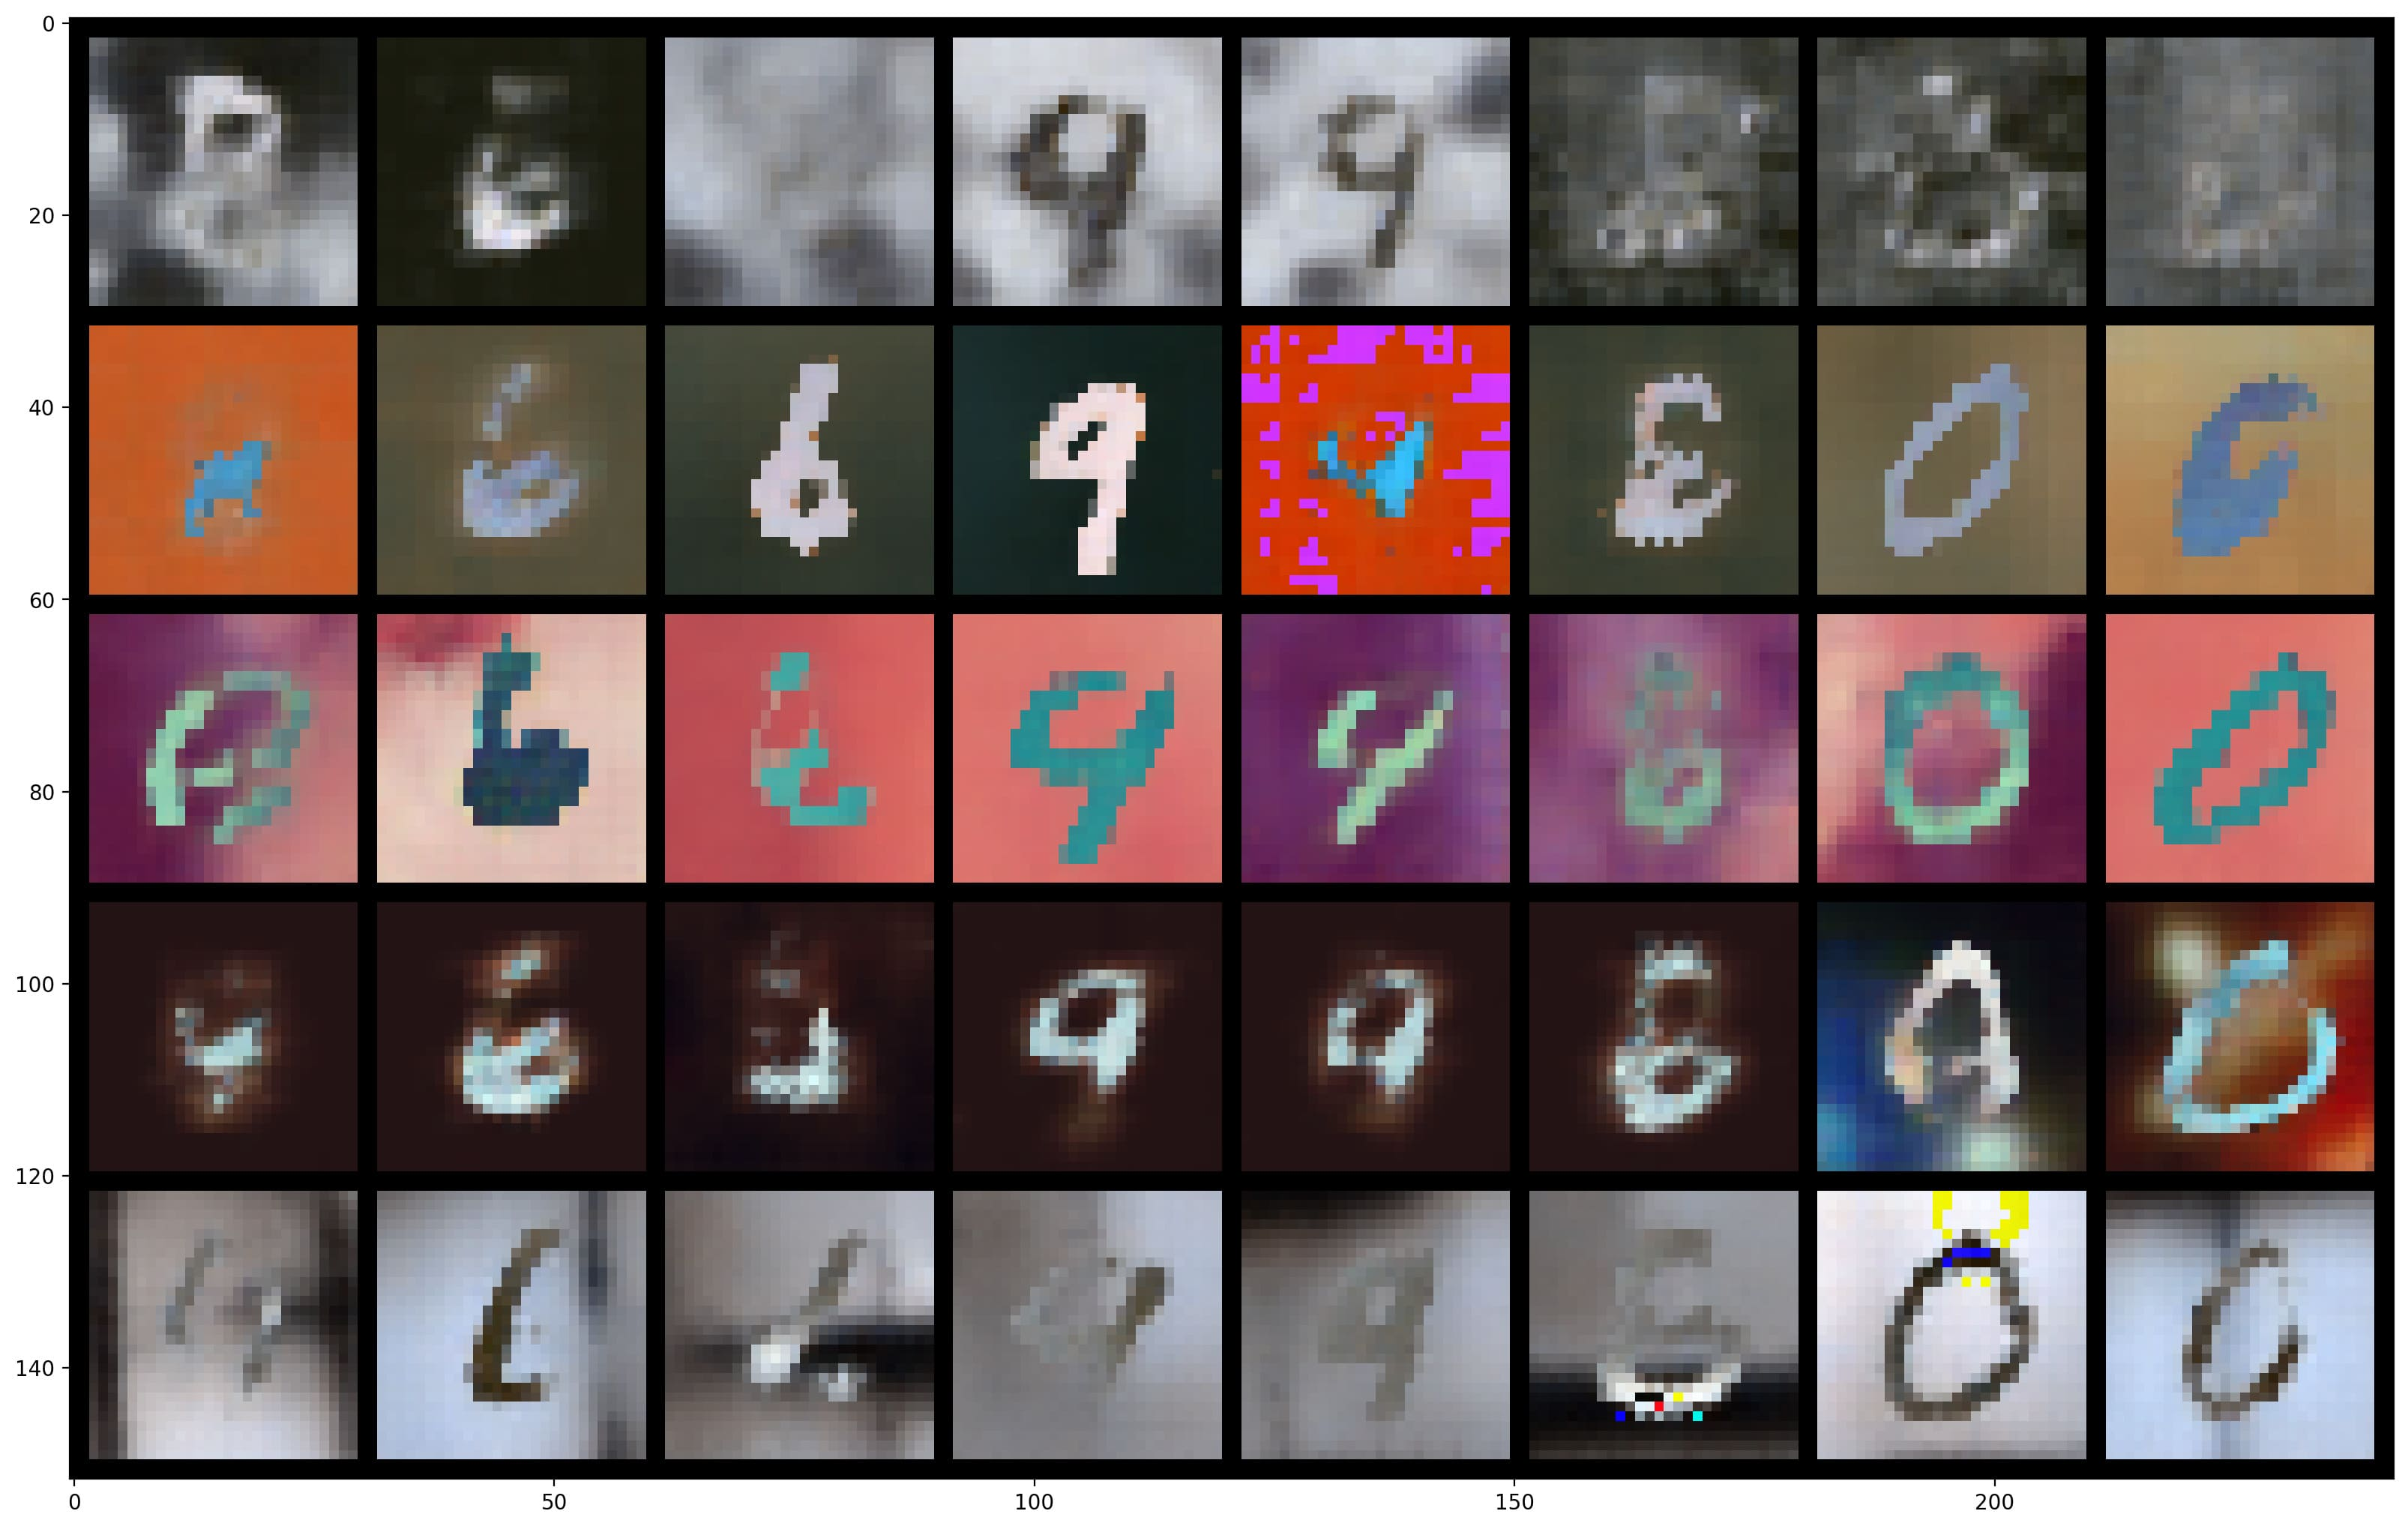
\includegraphics[width=\linewidth]{figures/datasets/mmnist/quali/mopoe_sampling}
         \caption*{\gls{MOPOE}}
     \end{subfigure} 
     
      \begin{subfigure}{0.25\textwidth}
         \centering
         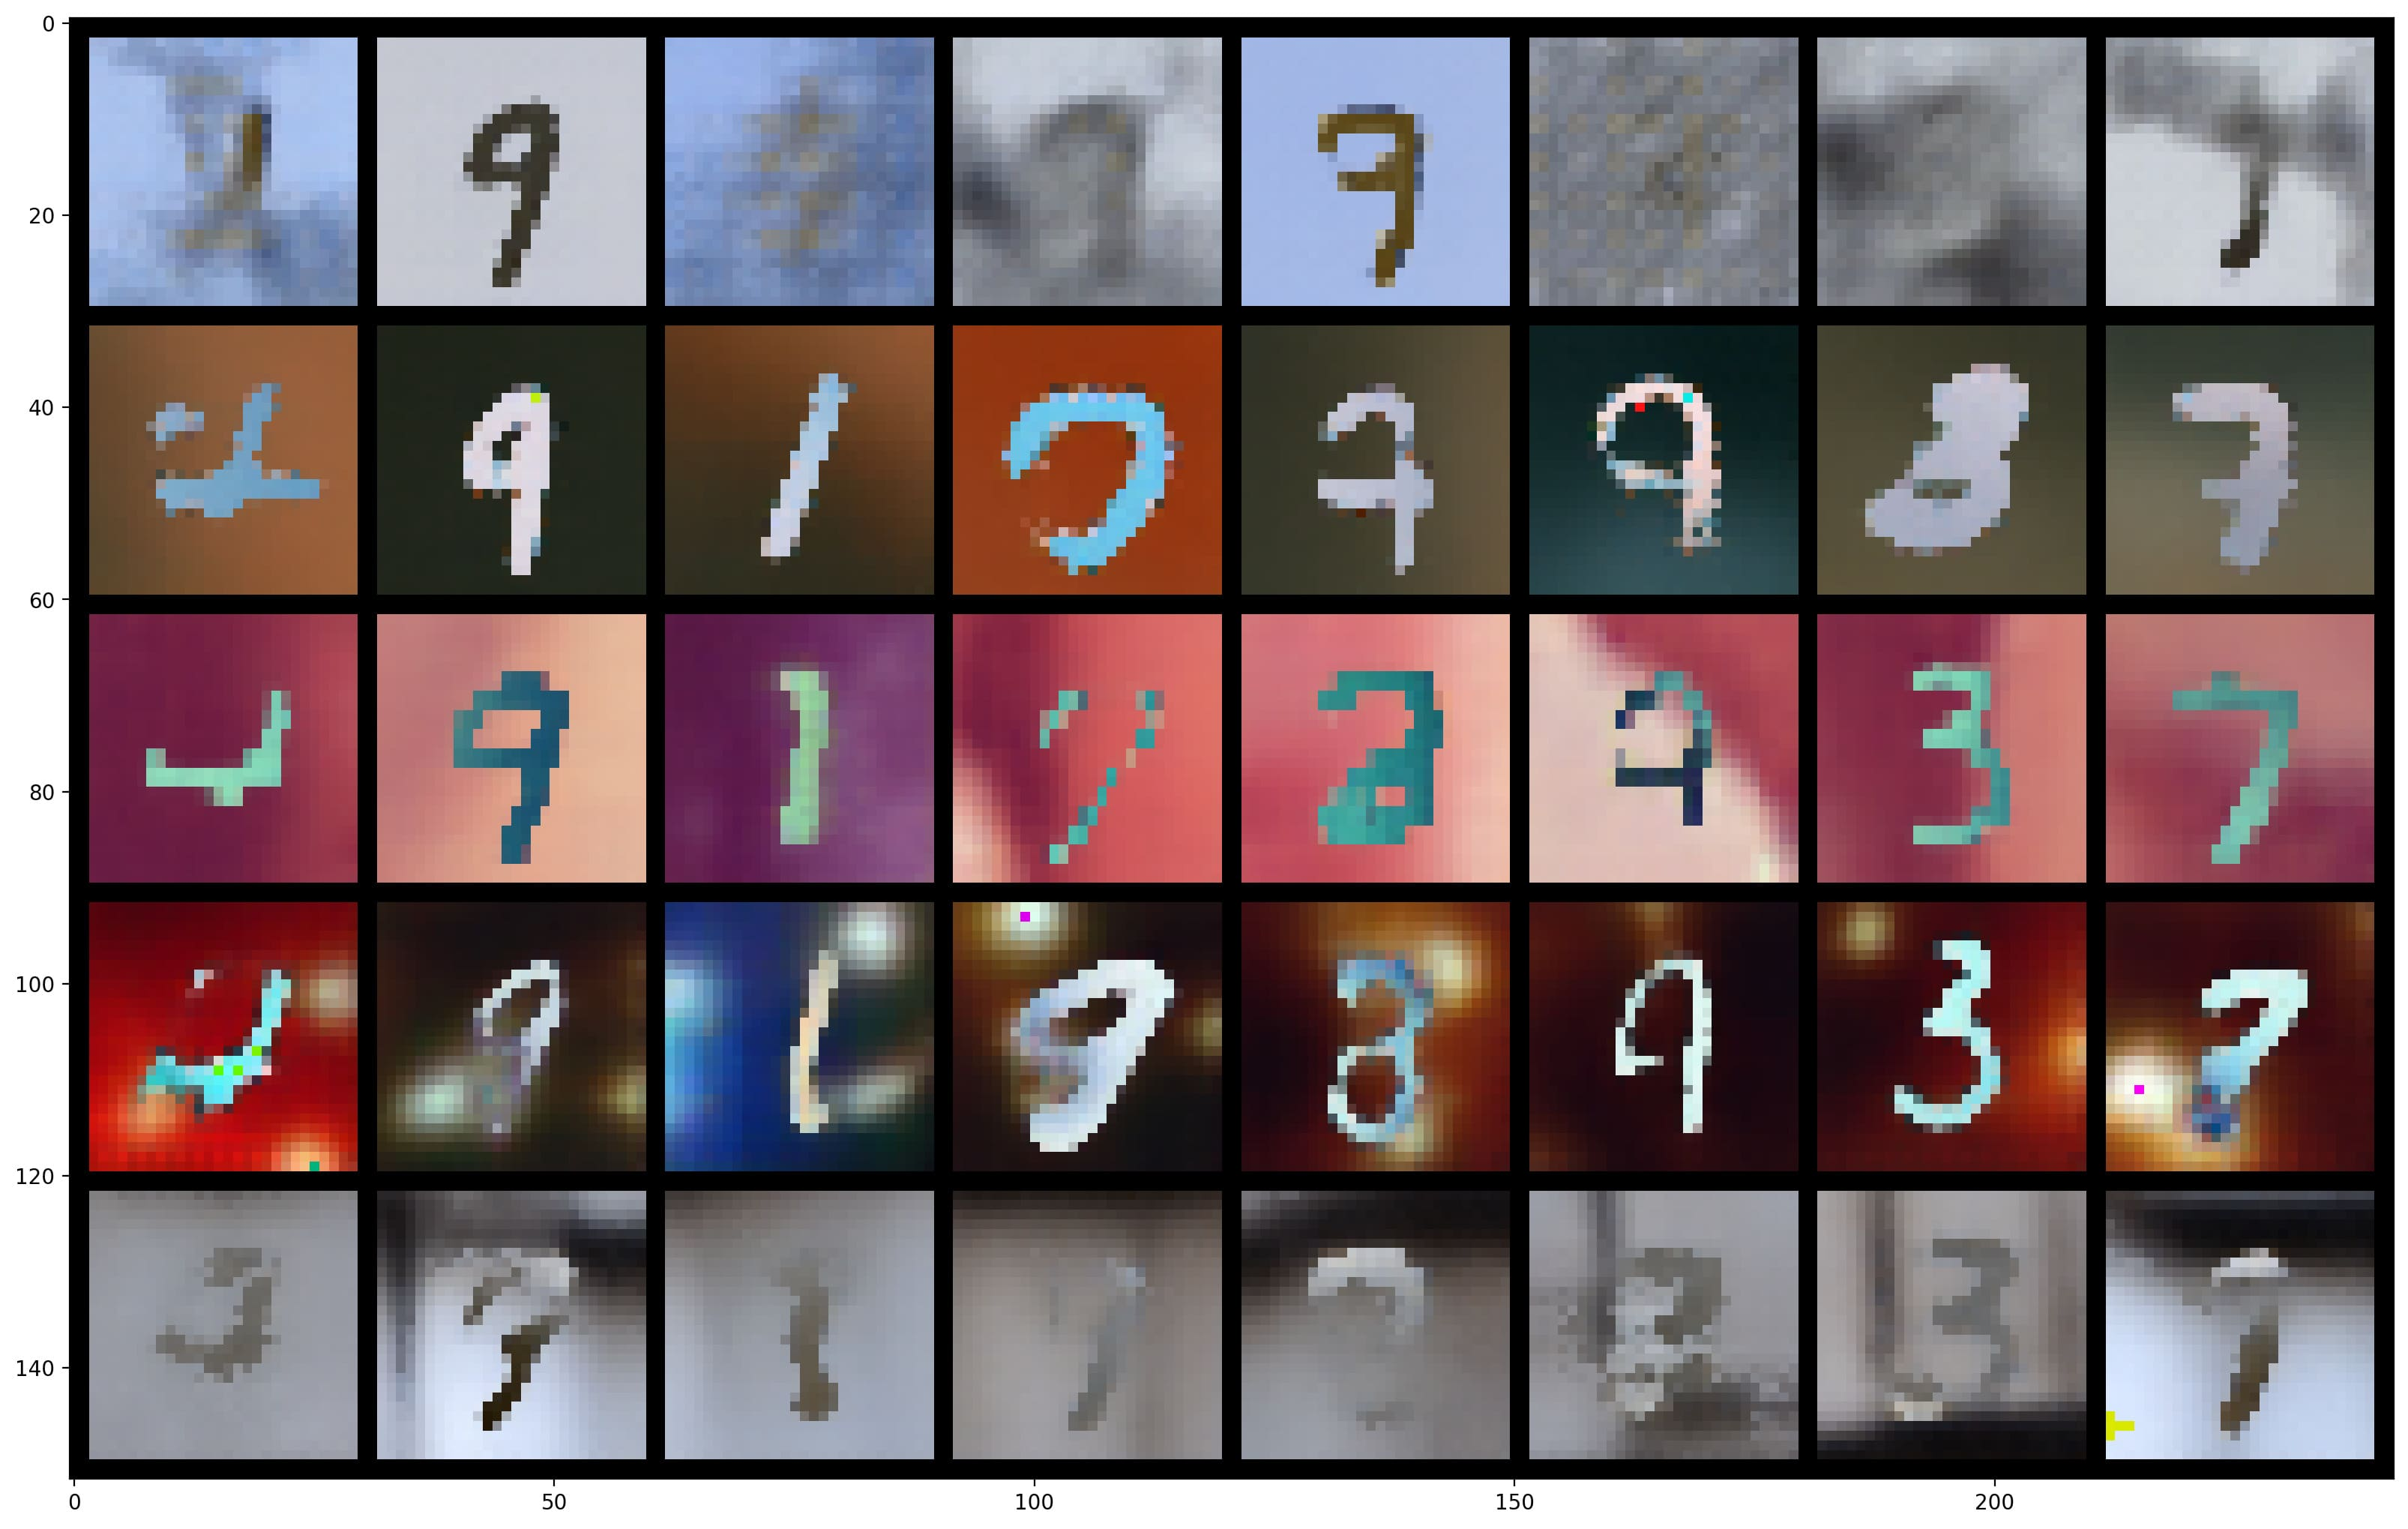
\includegraphics[width=\linewidth]{figures/datasets/mmnist/quali/nexus_sampling}
         \caption*{\gls{NEXUS}}
     
     \end{subfigure}
  \begin{subfigure}{0.25\textwidth}
         \centering
         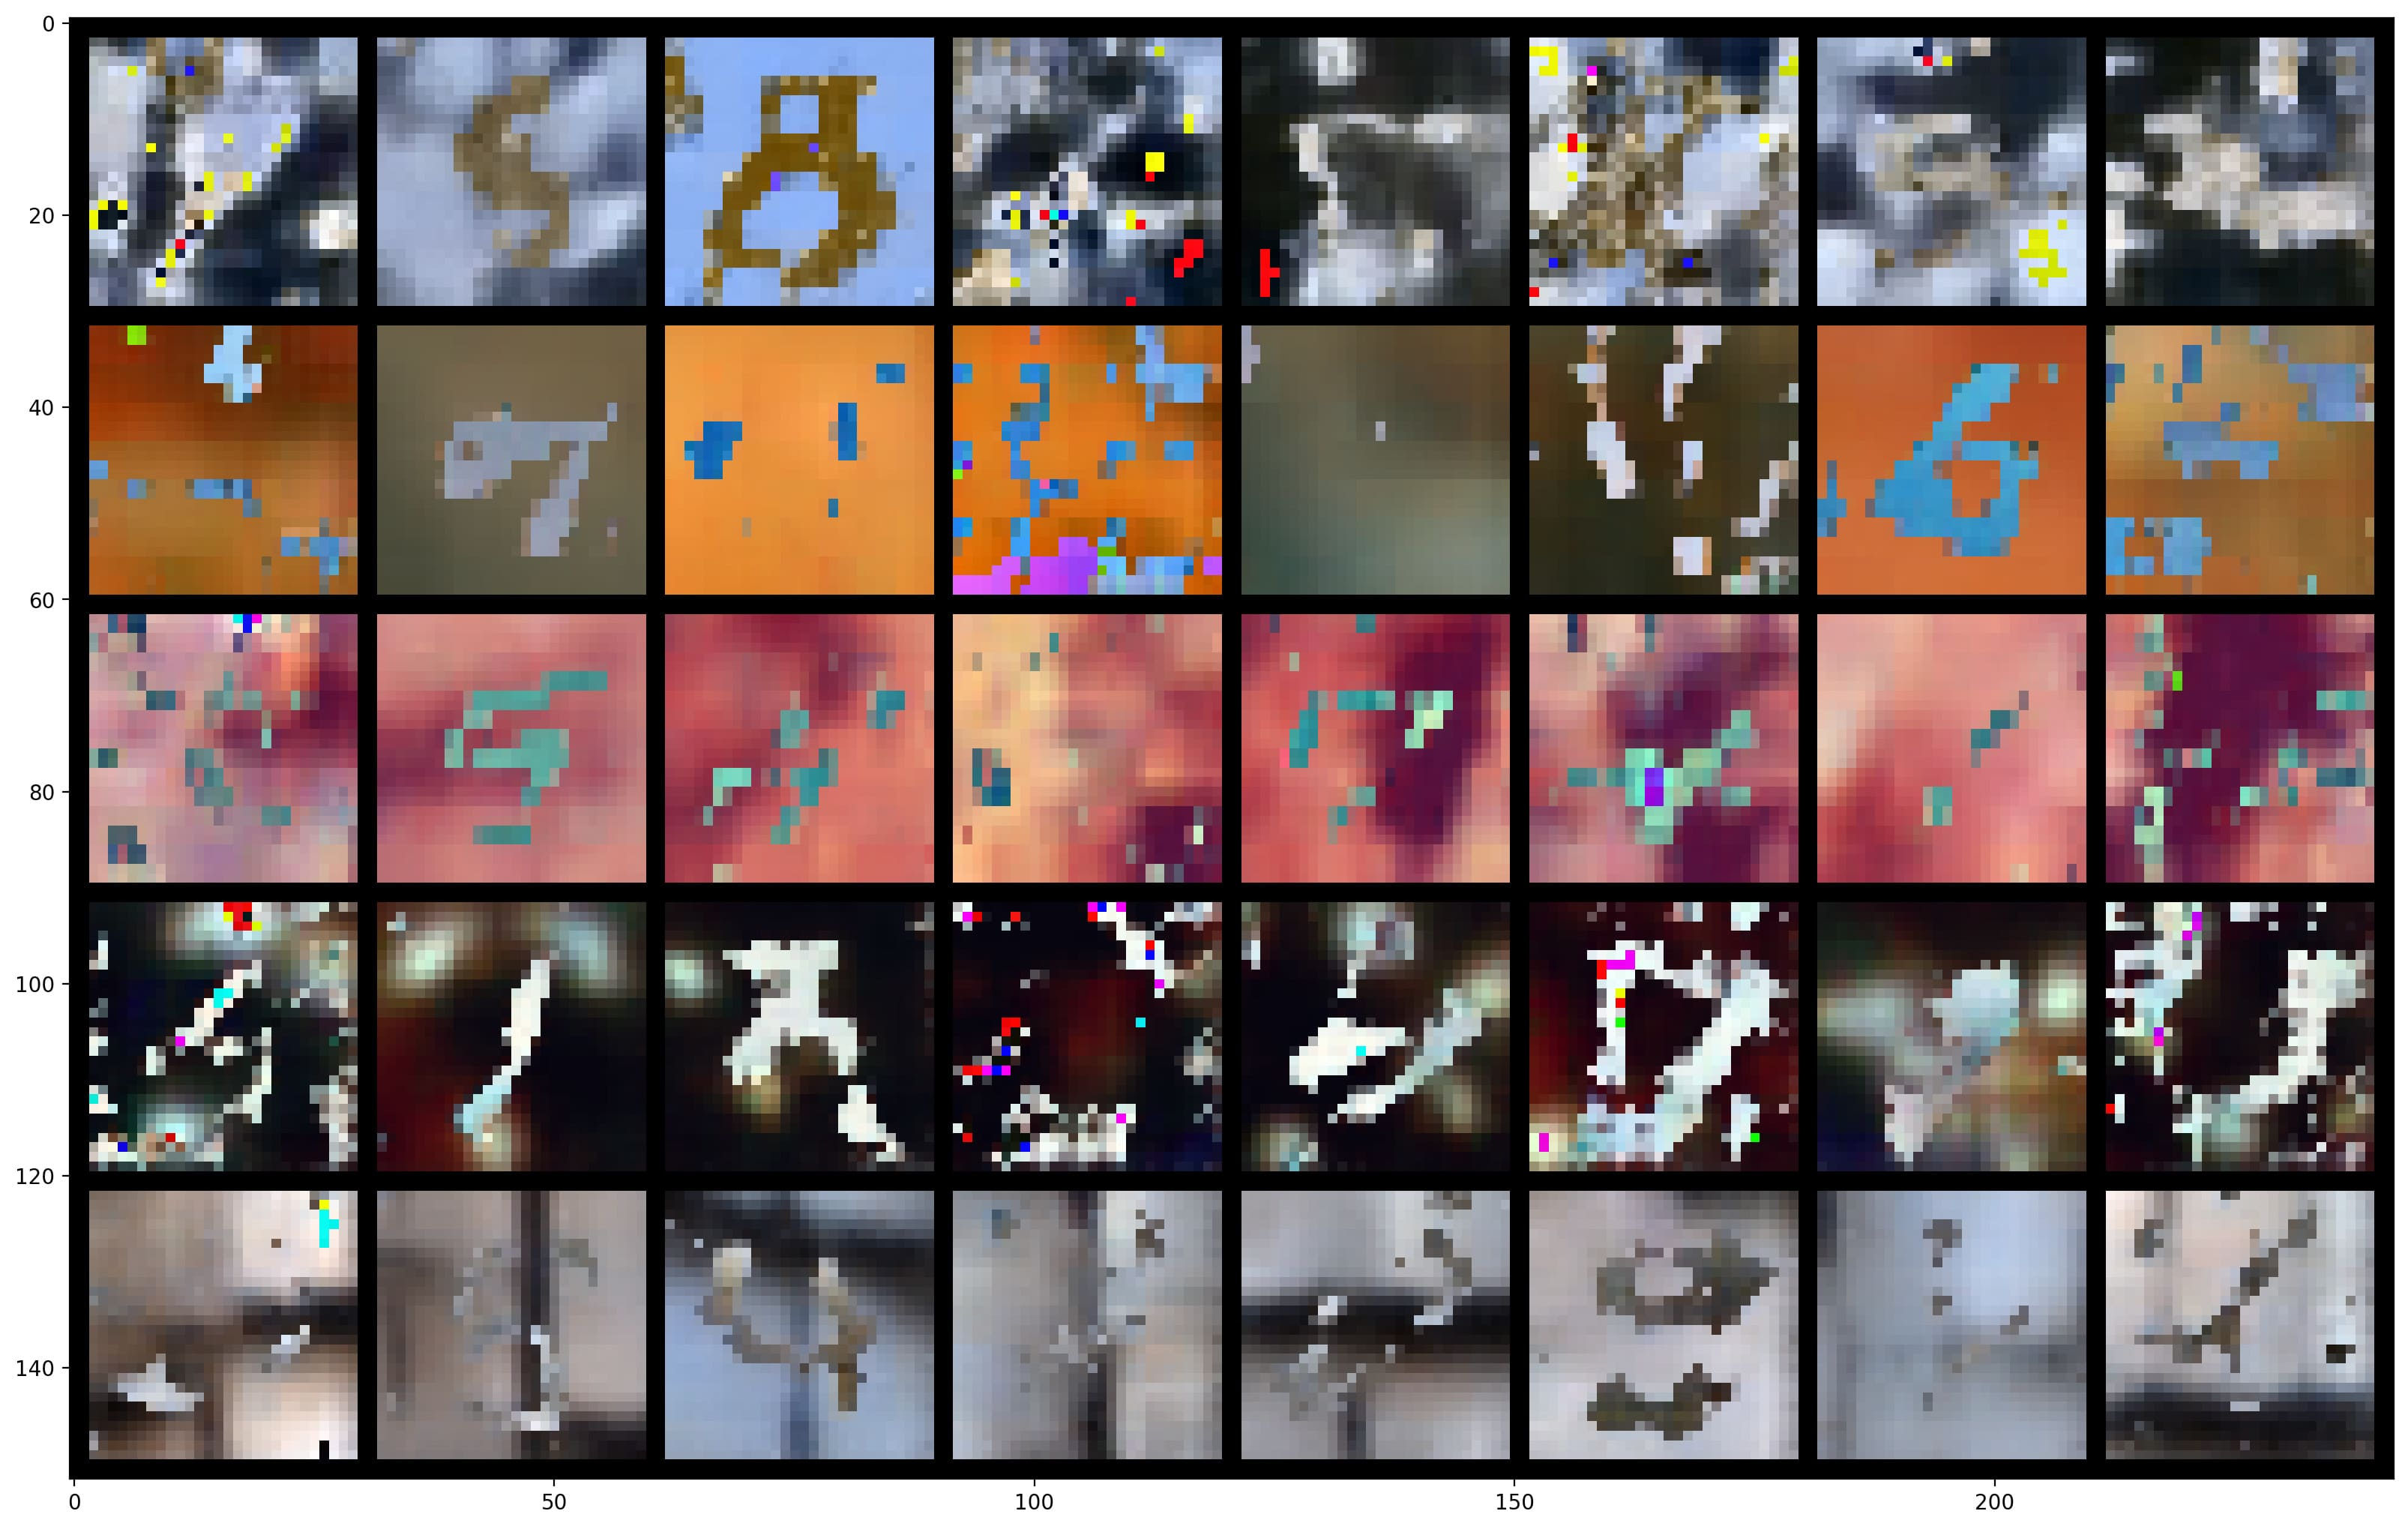
\includegraphics[width=\linewidth]{figures/datasets/mmnist/quali/mvtcae_sampling}
         \caption*{\gls{MVTCAE}}
   
     \end{subfigure}
  \begin{subfigure}{0.25\textwidth}
         \centering
         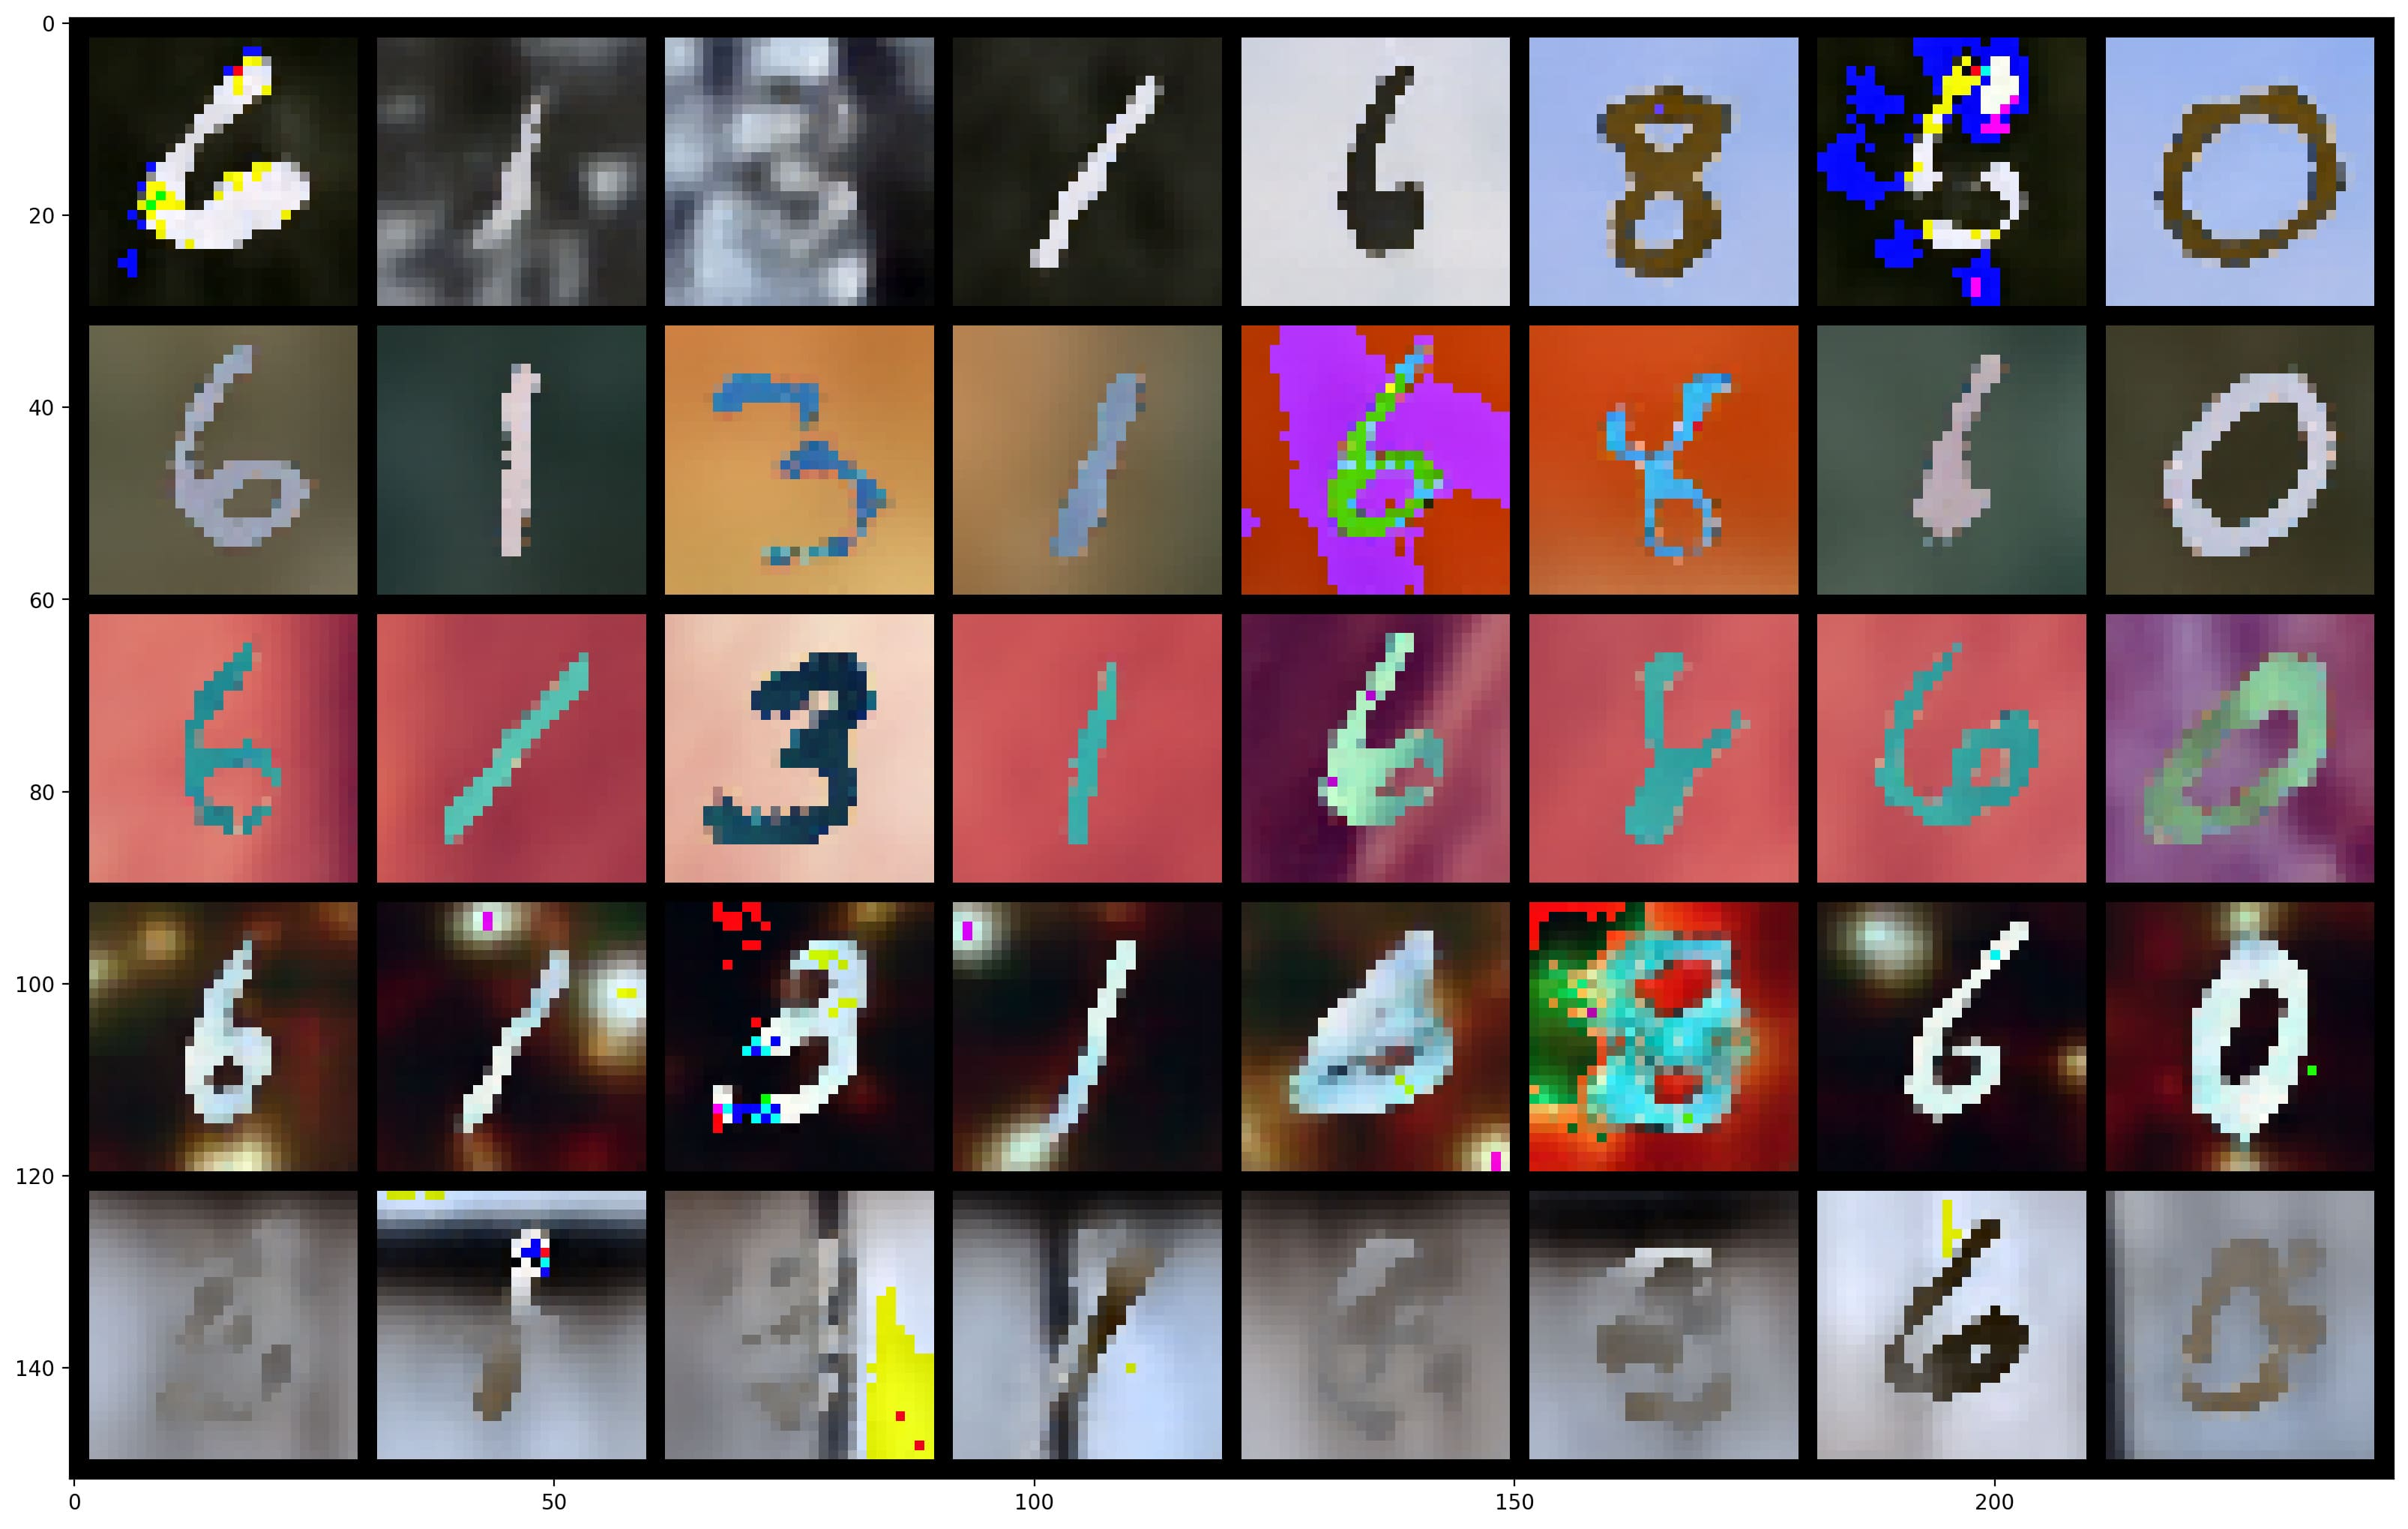
\includegraphics[page=1,width=\linewidth]{figures/datasets/mmnist/quali/MLD_sampling}
         \caption*{\textbf{\gls{MLD} (ours) }}
       
     \end{subfigure}
    
       \label{qual_mmnist}
\end{subfigure}
        \caption{Results for \textbf{\polymnist} data-set. \textit{Left}: a comparison of the generative coherence (\% $\uparrow$) and quality in terms of \gls{FID} ($\downarrow$) as a function of the number of inputs. We report the average performance following the leave-one-out strategy (see \ref{apdx:dataset_eval}).  \textit{Right}: are qualitative results for the joint generation of the 5 modalities.   }
        \label{fig:res_mmnist}
\end{figure}






\begin{figure}[hb]
\vspace*{-3mm}
     \centering
     \begin{subfigure}{0.16\textwidth}
         \centering
         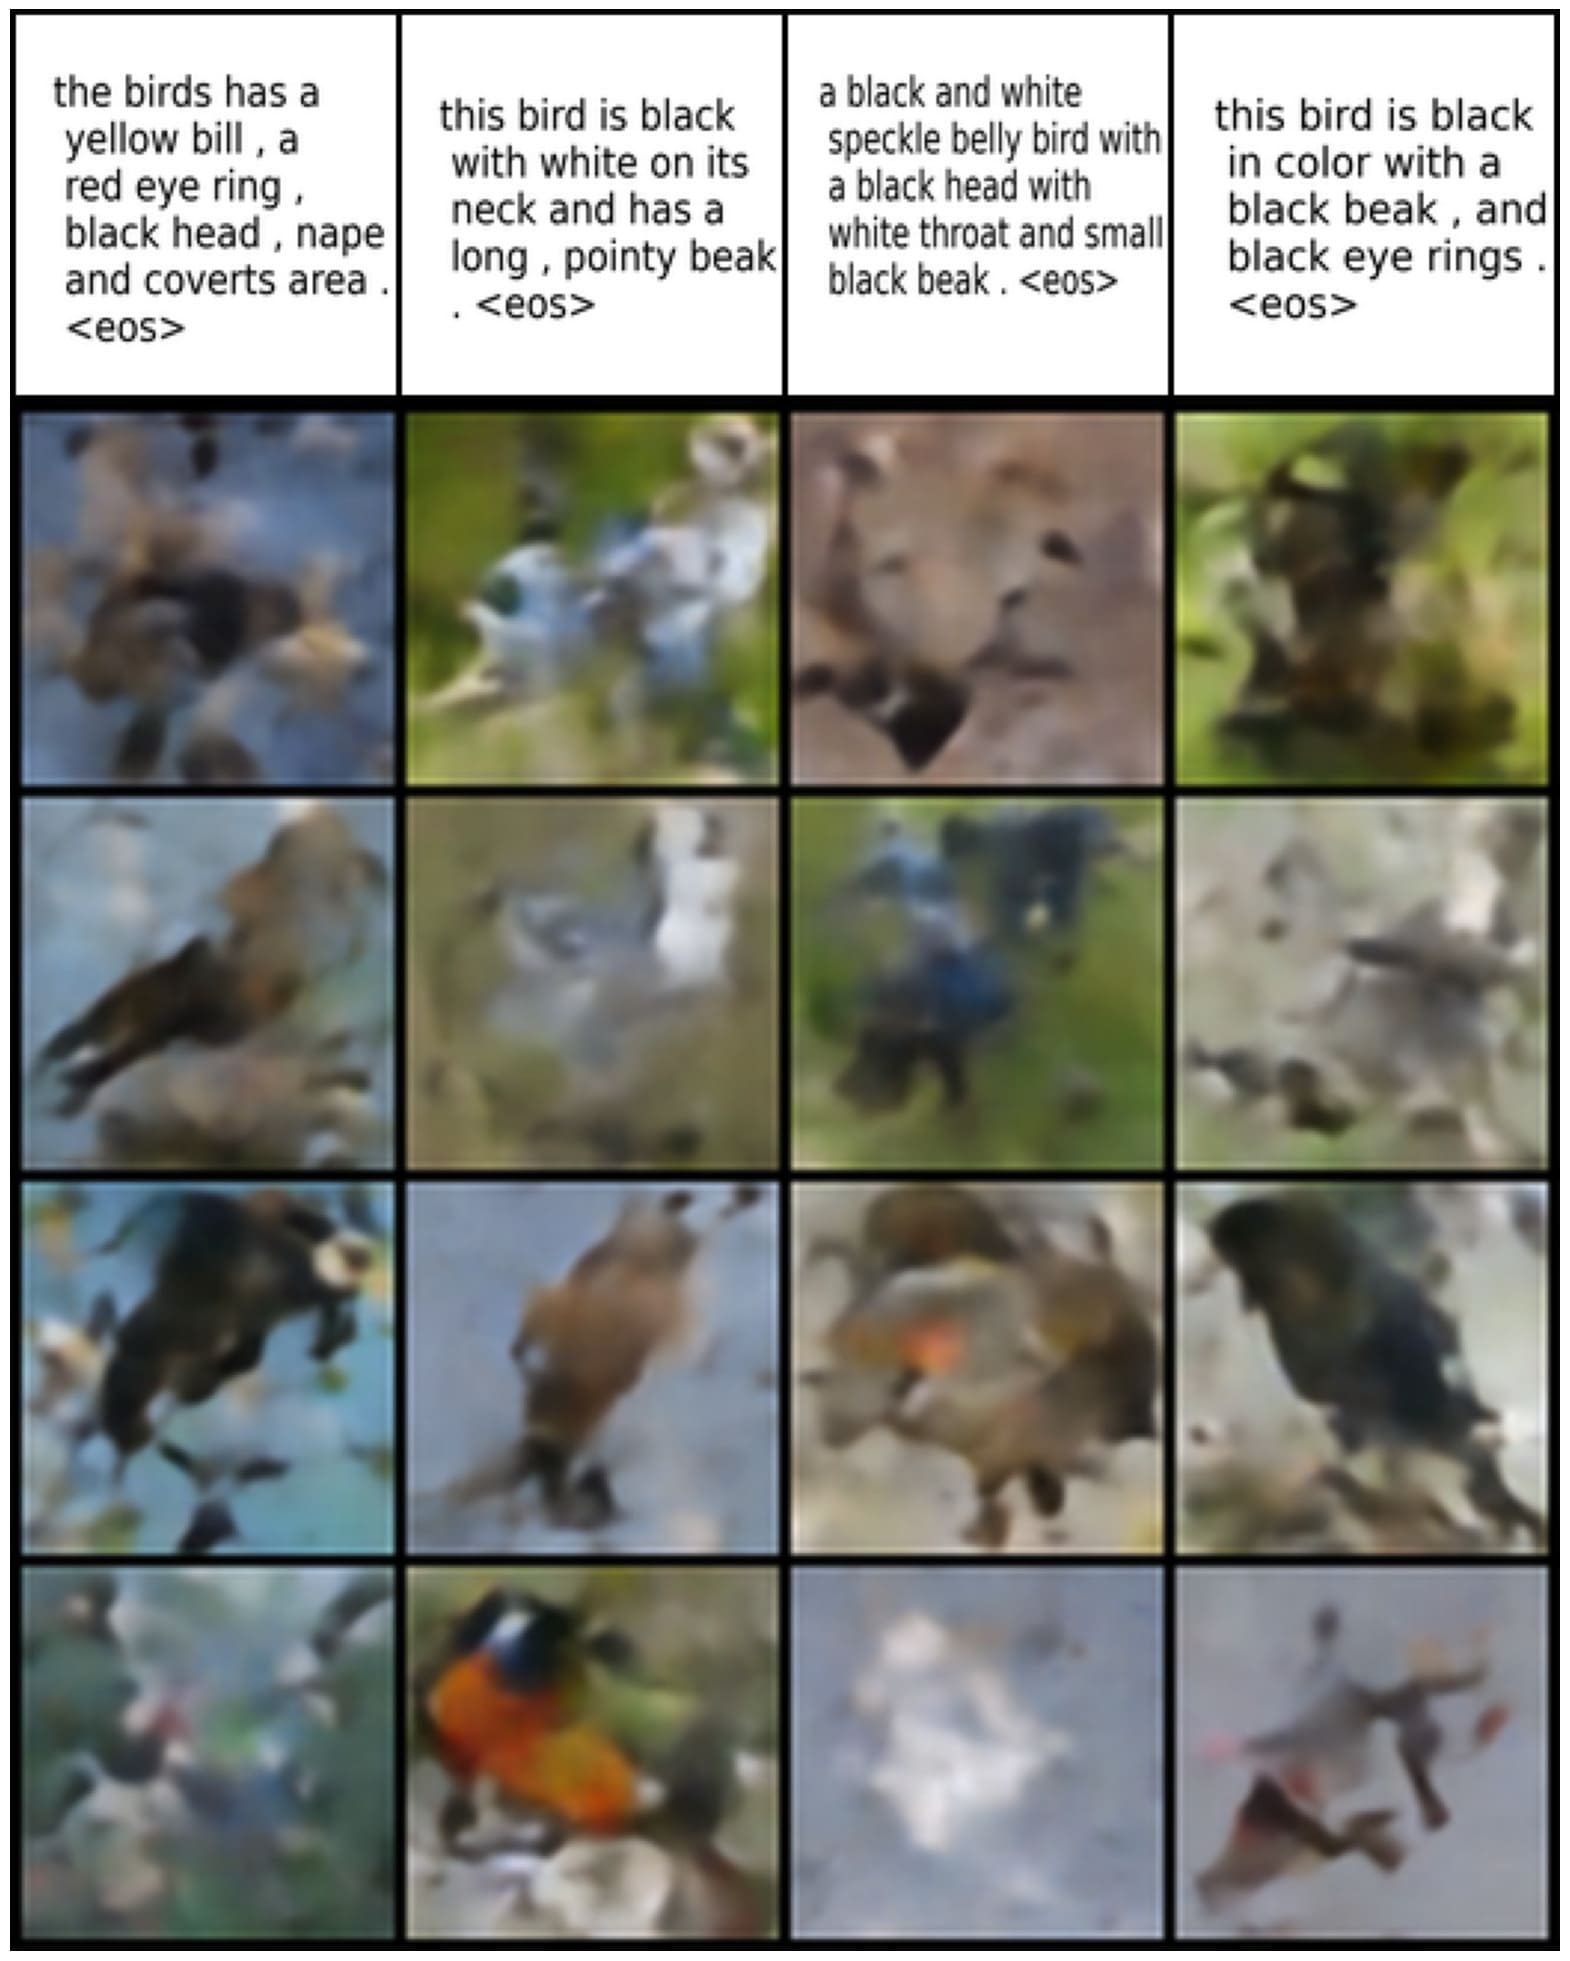
\includegraphics[width=\linewidth]{figures/datasets/cub/mvae_cond_text_image}
        \caption*{\gls{MVAE}}
        \end{subfigure}
   %  \begin{subfigure}{0.15\textwidth}
    %     \centering
    %     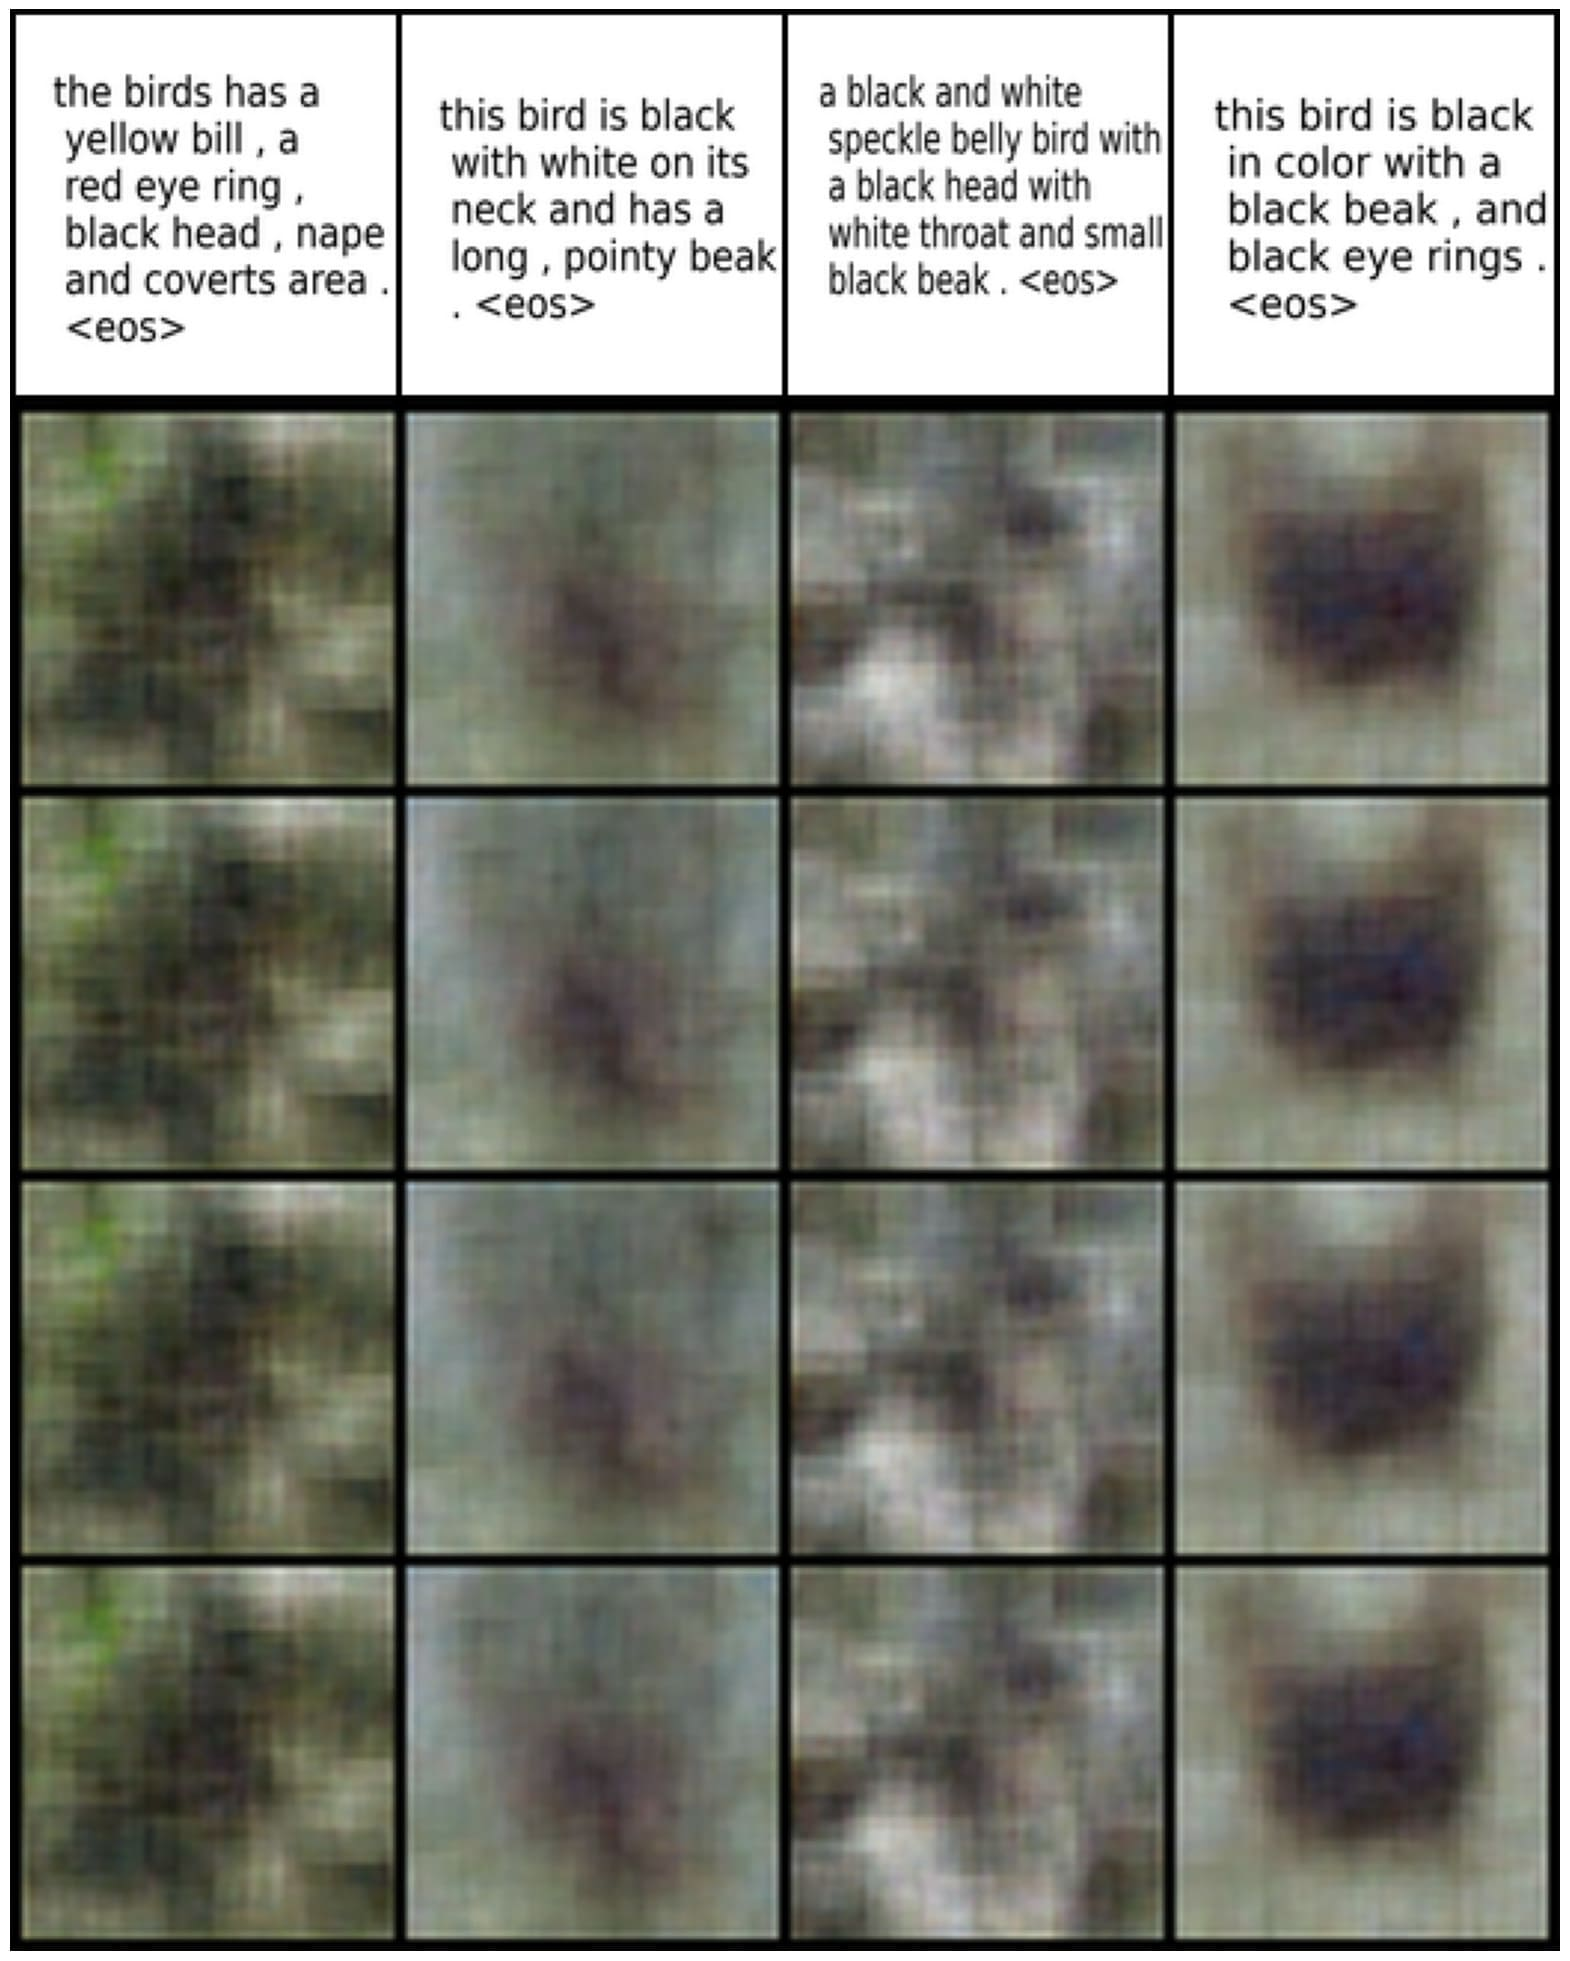
\includegraphics[width=\linewidth]{figures/datasets/cub/mmvae_cond_text_image}
    %     \caption*{\gls{MMVAE}} 
    % \end{subfigure}
       \begin{subfigure}{0.16\textwidth}
         \centering
         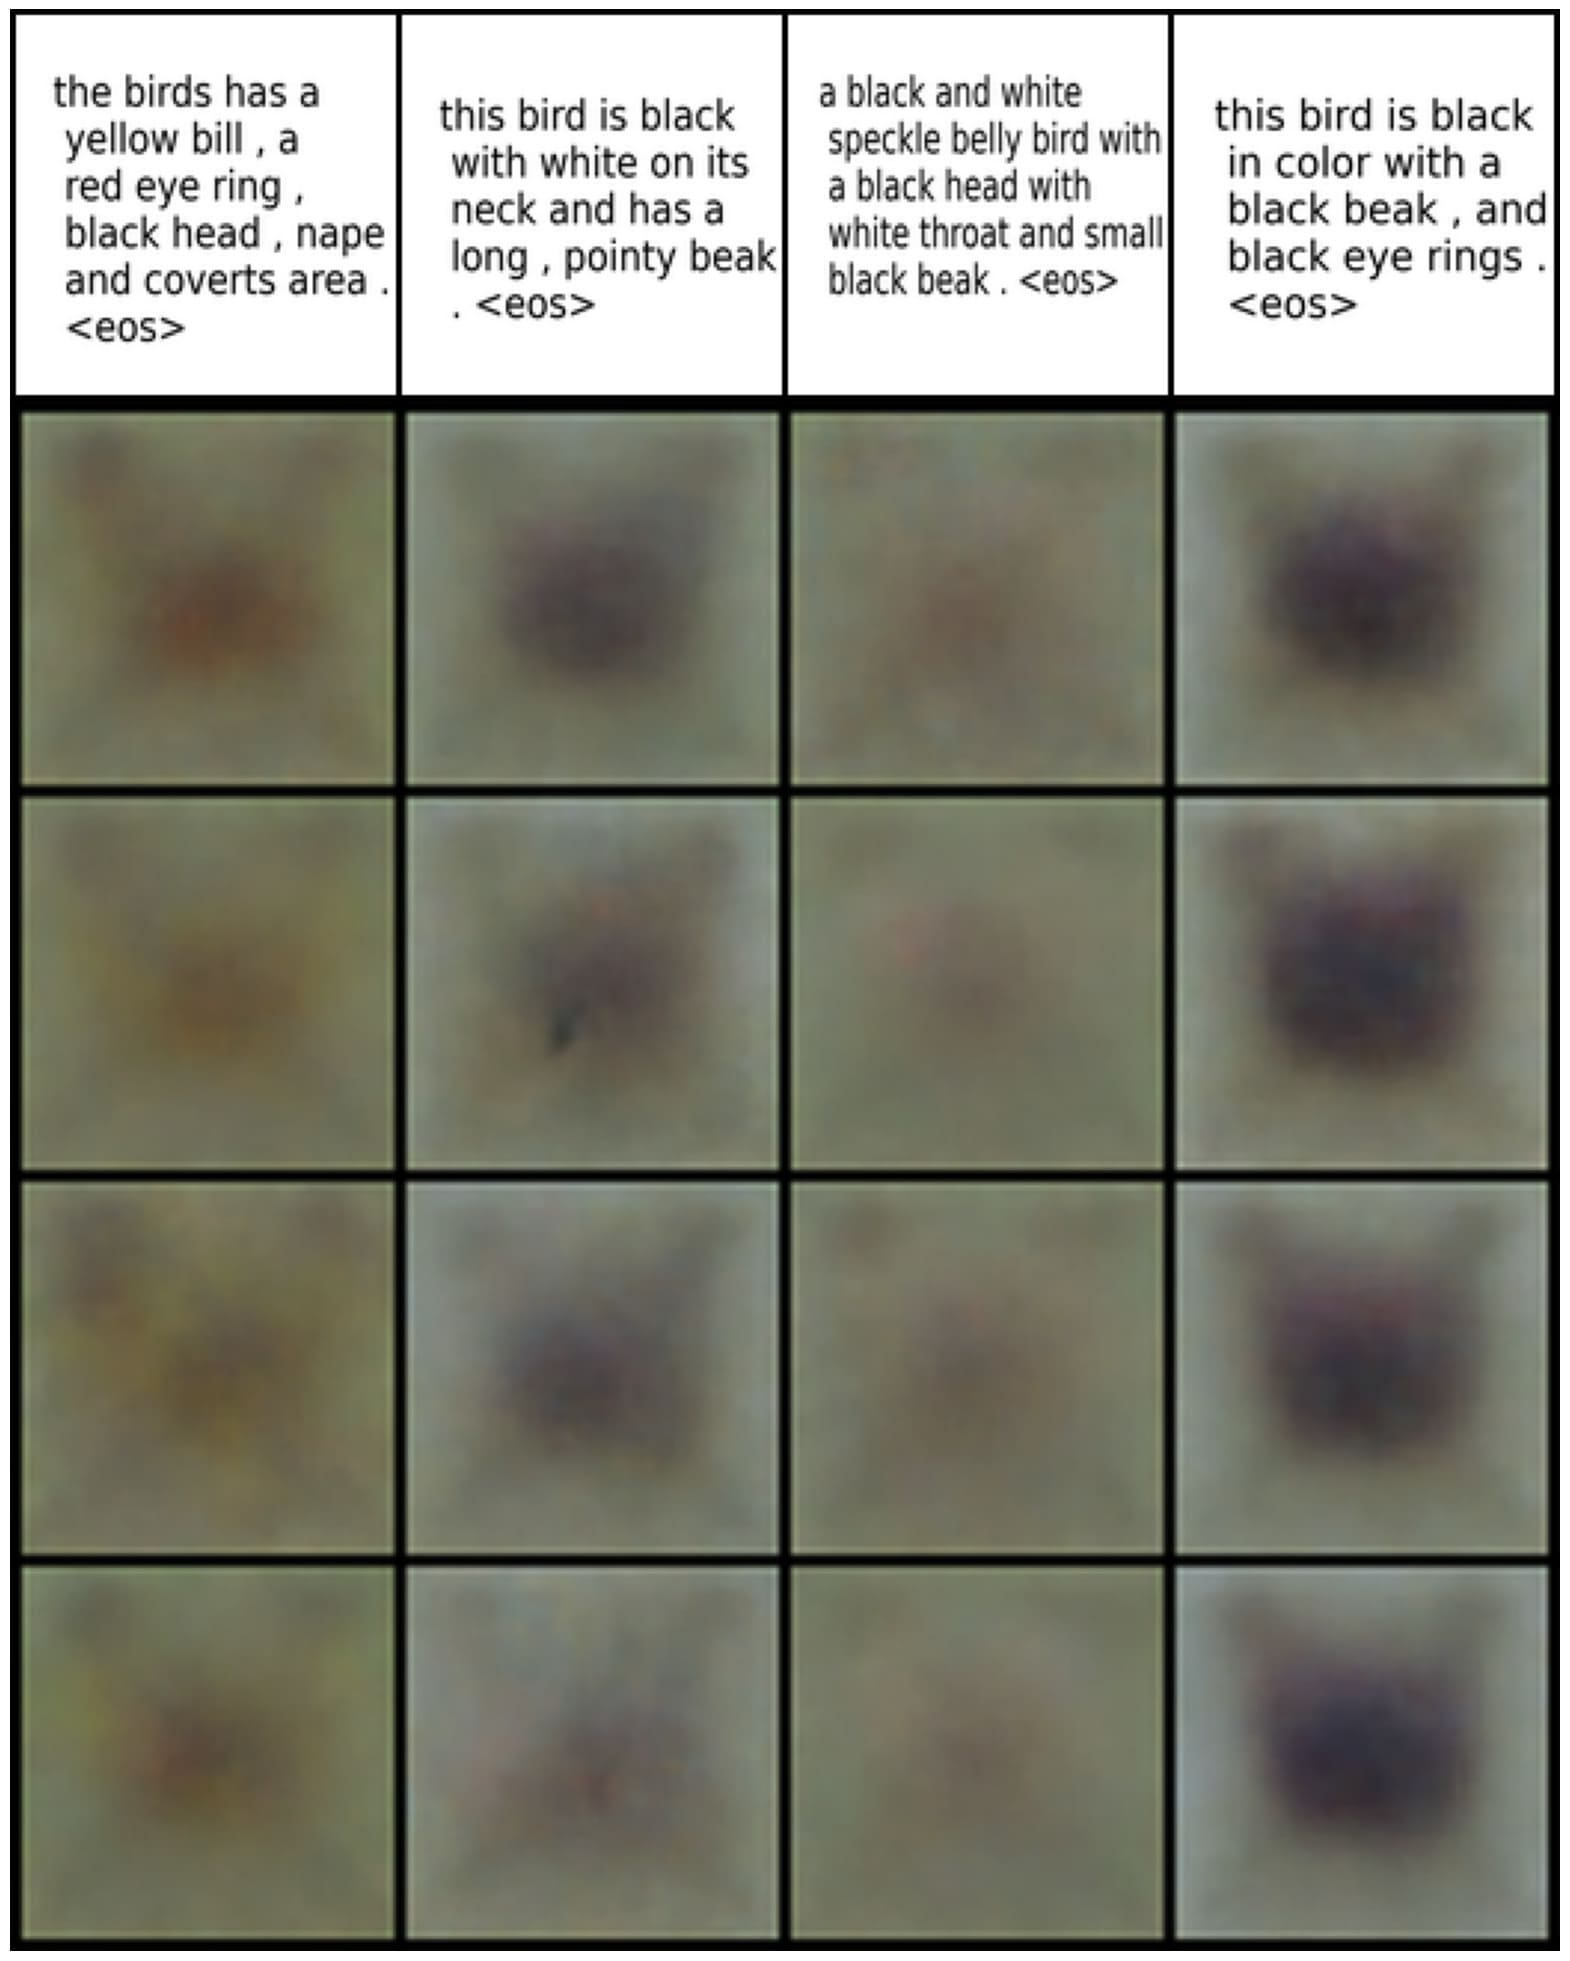
\includegraphics[width=\linewidth]{figures/datasets/cub/mopoe_cond_text_image}
         \caption*{\gls{MOPOE}}
     \end{subfigure}
     \begin{subfigure}{0.16\textwidth}
         \centering
         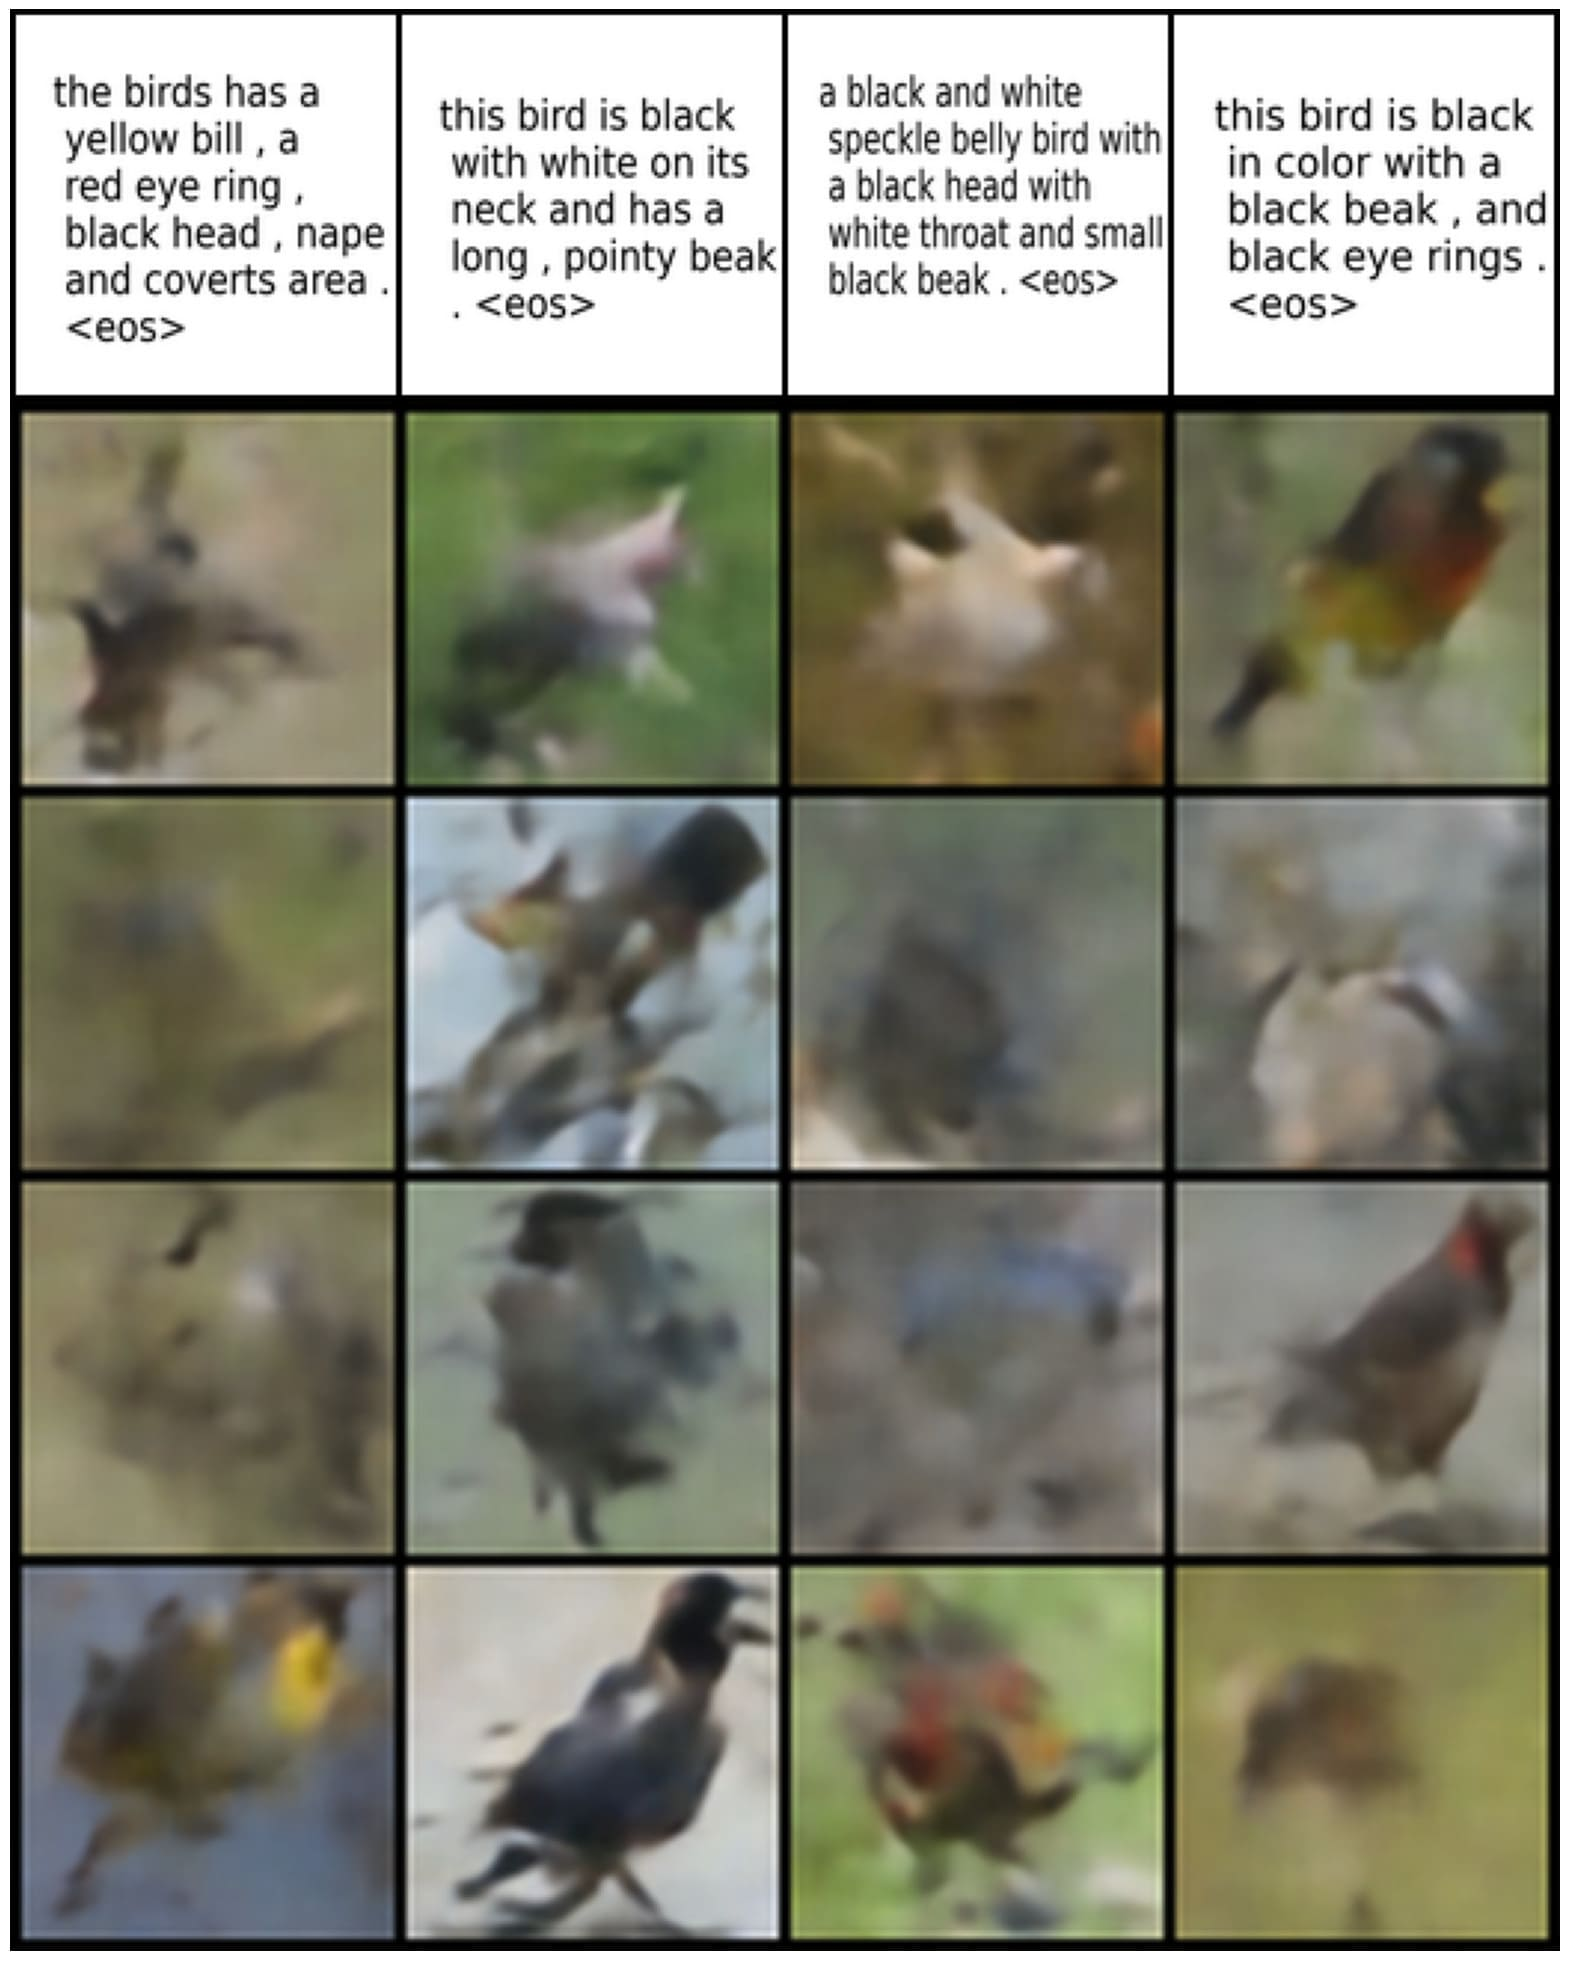
\includegraphics[width=\linewidth]{figures/datasets/cub/mvtcae_cond_text_image}
         \caption*{\gls{MVTCAE}}
     \end{subfigure}
  \begin{subfigure}{0.16\textwidth}
         \centering
         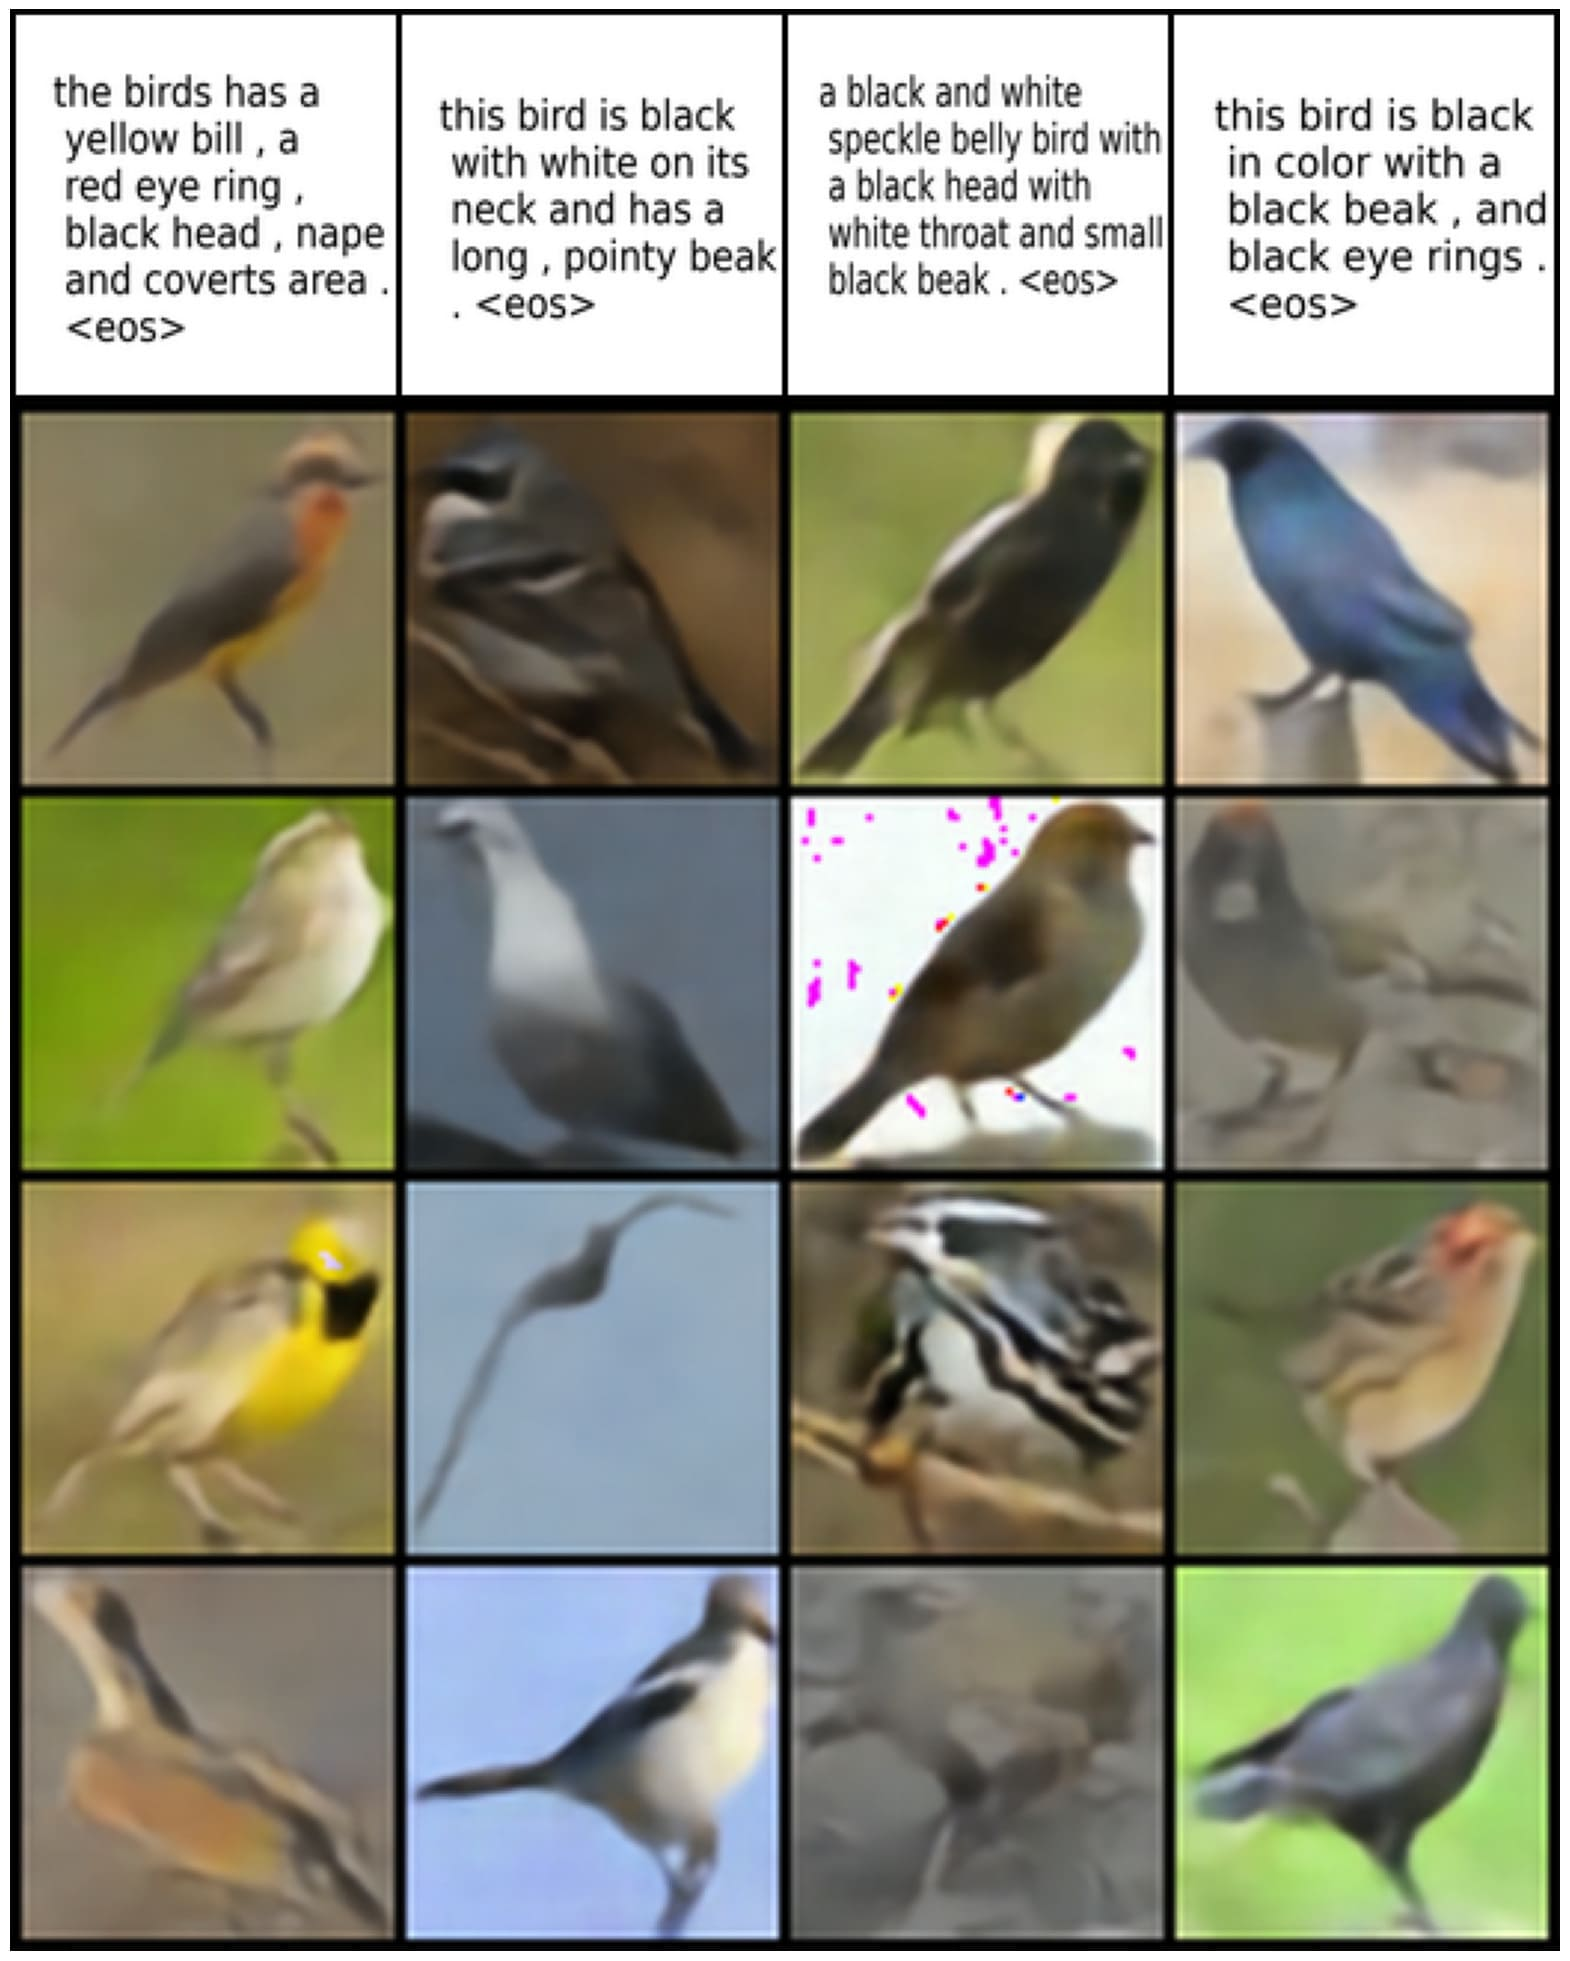
\includegraphics[page=1,width=\linewidth]{figures/datasets/cub/MLD_cond_text_image}
         \caption*{\textbf{\gls{MLD} (ours) }}
   \end{subfigure}
 \begin{subfigure}{0.16\textwidth}
         \centering
         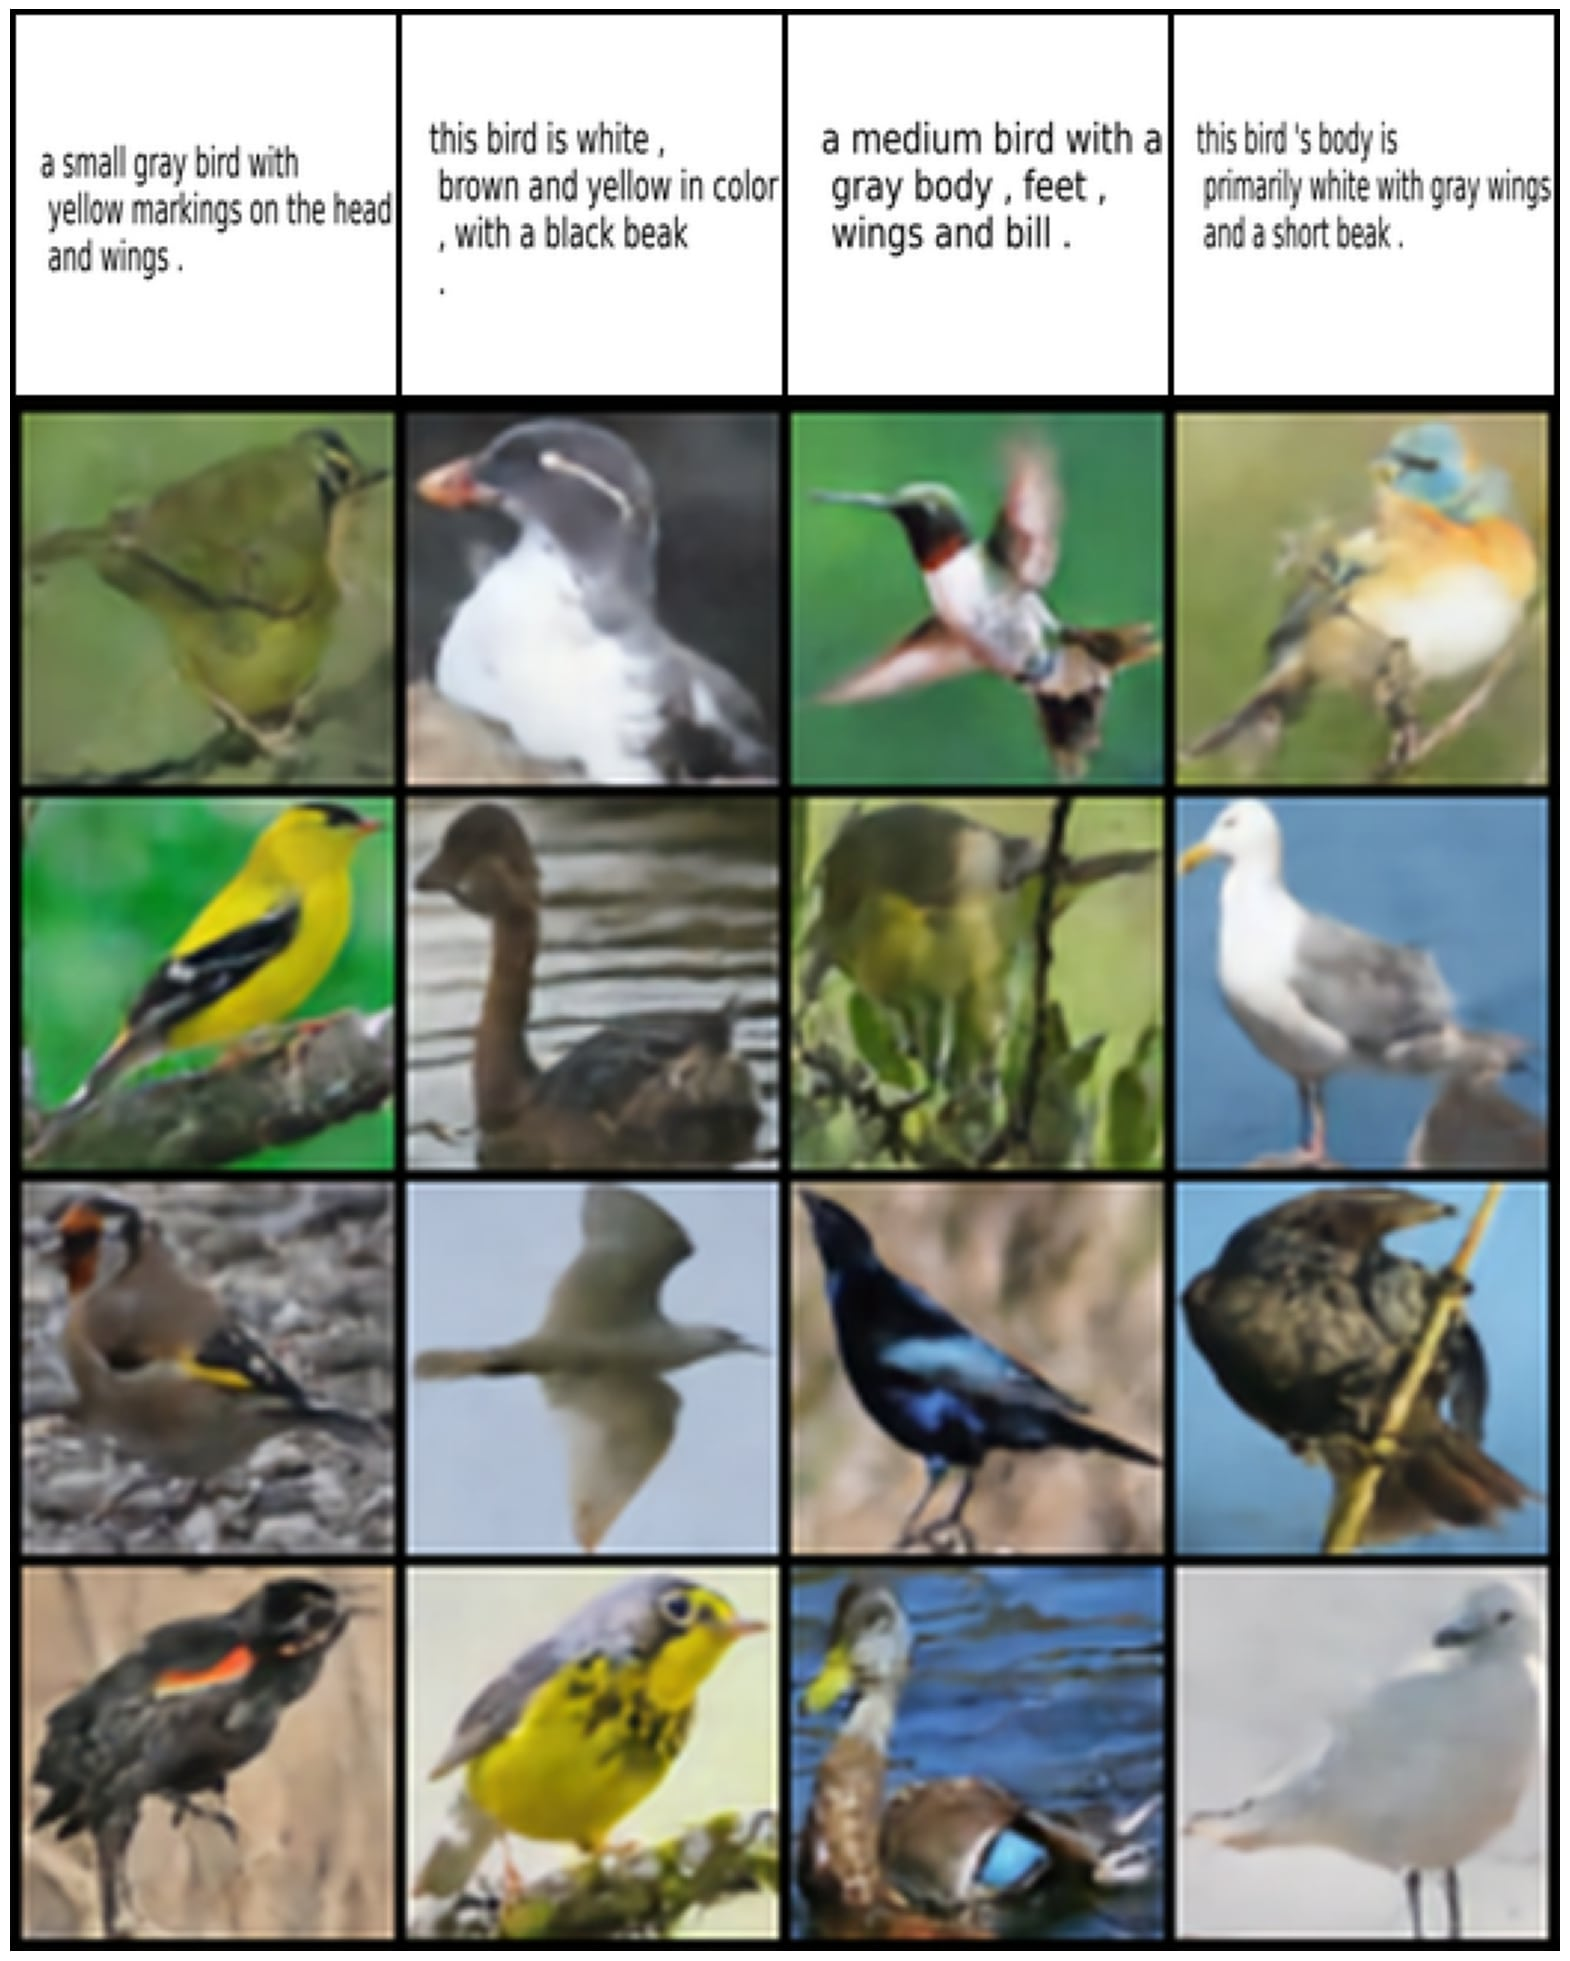
\includegraphics[page=1,width=\linewidth]{figures/datasets/cub/new_64/MLD_cond_text_image_mld64_new.jpg}
         
         \caption*{\textbf{\gls{MLD}* (ours)  }}
   \end{subfigure}
   %\vspace*{-1mm}
        \caption{Qualitative results on \textbf{\cub} data-set. Caption used as condition to generate the bird images. \textbf{MLD}* denotes the version of our method using a powerful image autoencoder. }
       \label{cap_image_cub}
        
\end{figure}






Finally, we explore the Caltech Birds \textbf{\cub} \citep{mmvaeShi2019} data-set, following the same experimentation protocol in \cite{Daunhawer2021} by using real bird images (instead of ResNet-features as in \cite{mmvaeShi2019}).  \Cref{cap_image_cub} presents qualitative results for caption to image conditional generation. 
\gls{MLD} is the only model capable of generating bird images with convincing coherence. Clearly, none of the \gls{VAE}-based methods is able to achieve sufficient caption to image conditional generation quality using the same simple autoencoder architecture. Note that an image autoencoder with larger capacity improves considerably \gls{MLD} generative performance, suggesting that careful engineering applied to modality specific autoencoders is a promising avenue for future work.
We report quantitative results in \ref{apdx:additionnal_res}, where we show generation quality \gls{FID} metric. Due to the unavailability of the labels in this data-set, coherence evaluation as with the previous data-sets is not possible. We then resort to \gls{CLIP-S} \cite{hessel2021clipscore} an image-captioning metric, that, despite its limitations for the considered data-set \cite{kim2022mutual}, shows that \gls{MLD} outperforms competitors.


